\documentclass{beamer}
\usetheme[sectionpage=progressbar, subsectionpage=progressbar, numbering=fraction, progressbar=foot, block=fill, background=light]{metropolis}
\usepackage{appendixnumberbeamer}
\usepackage{textpos}
\usepackage{booktabs}
\usepackage[scale=2]{ccicons}

\usepackage{pgfplots}
\usepgfplotslibrary{dateplot}
\usetikzlibrary{backgrounds}
\usepackage{xspace}
\newcommand{\themename}{\textbf{\textsc{metropolis}}\xspace}
\title{Attention based models in End-to-End ASR}
\subtitle{Exploration of Attention in ESPNET toolkit}
\date{\today}
\author{Shreekantha Nadig}
\institute{International Institute of Information Technology - Bangalore}
%\titlegraphic{\hfill\includegraphics[height=1.5cm]{logo.pdf}}

\usepackage{tikz}
\usetikzlibrary{shapes,shadows,arrows,patterns, matrix}

\tikzstyle{line} = [draw, -latex']
\tikzstyle{round} = [draw, circle, fill=black!30, minimum size=4em, node distance=4em, font=\fontsize{30}{10}\selectfont]
\tikzstyle{mlp_enc} = [rectangle, draw, fill=red!50, text width=2cm, minimum height=5em, text centered, node distance=10em, font=\fontsize{20}{10}\selectfont]
\tikzstyle{mlp_att} = [rectangle, draw, fill=green!50, text width=2cm, minimum height=5em, text centered, node distance=10em, font=\fontsize{20}{10}\selectfont]
\tikzstyle{mlp_dec} = [rectangle, draw, fill=blue!50, text width=2cm, minimum height=5em, text centered, node distance=10em, font=\fontsize{20}{10}\selectfont]
\tikzstyle{enc_h} = [rectangle, draw,  pattern=horizontal lines, pattern color=red!60, text width=1cm, minimum height=10em, minimum width=3em, text centered, node distance=10em, font=\fontsize{25}{10}\selectfont]
\tikzstyle{atts} = [rectangle, draw,  pattern=horizontal lines, pattern color=green!70, text width=1cm, minimum height=10em, minimum width=3em, text centered, node distance=10em, font=\fontsize{20}{10}\selectfont]
\tikzstyle{dec_z} = [rectangle, draw,  pattern=horizontal lines, pattern color=blue!60, text width=1cm, minimum height=10em, minimum width=3em, text centered, node distance=10em, font=\fontsize{20}{10}\selectfont]
\tikzstyle{cnn} = [rectangle, draw,  pattern=crosshatch, pattern color=red!50!blue!50, text width=2cm, minimum height=5em, text centered, node distance=10em, font=\fontsize{20}{10}\selectfont]
\tikzstyle{box} = [rectangle, draw,  fill=blue!20, text width=3cm, minimum height=5em, minimum width=3em, text centered, node distance=10em, font=\fontsize{20}{10}\selectfont]

\begin{document}
	\addtobeamertemplate{frametitle}{}{%
			\begin{textblock*}{100mm}(.97\textwidth,-1cm)
				{
\includegraphics[width=2.5em]{iiitb_logo.png}}
		\end{textblock*}}
	
\maketitle

\begin{frame}{Table of contents}
\begin{scriptsize}
\setbeamertemplate{section in toc}[sections numbered]
\tableofcontents[hideallsubsections]
\end{scriptsize}
\end{frame}

\section{Introduction}
\begin{frame}[fragile]{BLSTM}
	\begin{center}
	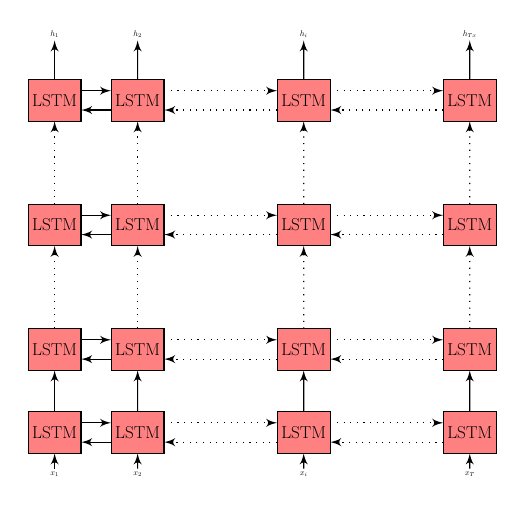
\begin{tikzpicture}[scale=0.3, every node/.style={transform shape}]
			\onslide<1->\node[mlp_enc](LSTM_1_1){LSTM};
			\node[mlp_enc, right of=LSTM_1_1](LSTM_1_2) {LSTM};
			\path [line] (LSTM_1_1.20) to (LSTM_1_1.20-|LSTM_1_2.west);
			\path [line] (LSTM_1_2.200) to (LSTM_1_2.-20-|LSTM_1_1.east);     
			
			\node[mlp_enc, right of=LSTM_1_2, node distance = 20em](LSTM_1_i) {LSTM};
			\path [line, dotted] (LSTM_1_2.20) to (LSTM_1_2.20-|LSTM_1_i.west);
			\path [line, dotted] (LSTM_1_i.200) to (LSTM_1_i.200-|LSTM_1_2.east);
			
			\node[mlp_enc, right of=LSTM_1_i, node distance = 20em](LSTM_1_Tx) {LSTM};
			\path [line, dotted] (LSTM_1_i.20) to (LSTM_1_i.20-|LSTM_1_Tx.west);
			\path [line, dotted] (LSTM_1_Tx.200) to (LSTM_1_Tx.200-|LSTM_1_i.east);
			
			\node [below of=LSTM_1_1, node distance = 5em] (x1) {$x_{1}$};
			\node [below of=LSTM_1_2, node distance = 5em] (x2) {$x_{2}$};
			\node [below of=LSTM_1_i, node distance = 5em] (xi) {$x_{i}$};
			\node [below of=LSTM_1_Tx, node distance = 5em] (xTx) {$x_{T}$};
			
			\path [line] (x1) to (LSTM_1_1);
			\path [line] (x2) to (LSTM_1_2);
			\path [line] (xi) to (LSTM_1_i);
			\path [line] (xTx) to (LSTM_1_Tx);
			
			\onslide<2->\node[mlp_enc, above of = LSTM_1_1](LSTM_2_1){LSTM};
			\node[mlp_enc, right of=LSTM_2_1](LSTM_2_2) {LSTM};
			\path [line] (LSTM_2_1.20) to (LSTM_2_1.20-|LSTM_2_2.west);
			\path [line] (LSTM_2_2.200) to (LSTM_2_2.-20-|LSTM_2_1.east);     
			
			\node[mlp_enc, right of=LSTM_2_2, node distance = 20em](LSTM_2_i) {LSTM};
			\path [line, dotted] (LSTM_2_2.20) to (LSTM_2_2.20-|LSTM_2_i.west);
			\path [line, dotted] (LSTM_2_i.200) to (LSTM_2_i.200-|LSTM_2_2.east);
			
			\node[mlp_enc, right of=LSTM_2_i, node distance = 20em](LSTM_2_Tx) {LSTM};
			\path [line, dotted] (LSTM_2_i.20) to (LSTM_2_i.20-|LSTM_2_Tx.west);
			\path [line, dotted] (LSTM_2_Tx.200) to (LSTM_2_Tx.200-|LSTM_2_i.east);
			
			\path [line] (LSTM_1_1) to (LSTM_2_1);
			\path [line] (LSTM_1_2) to (LSTM_2_2);
			\path [line] (LSTM_1_i) to (LSTM_2_i);
			\path [line] (LSTM_1_Tx) to (LSTM_2_Tx);
			
			\node[mlp_enc, above of = LSTM_2_1, node distance = 15em](LSTM_i_1){LSTM};
			\node[mlp_enc, right of=LSTM_i_1](LSTM_i_2) {LSTM};
			\path [line] (LSTM_i_1.20) to (LSTM_i_1.20-|LSTM_i_2.west);
			\path [line] (LSTM_i_2.200) to (LSTM_i_2.-20-|LSTM_i_1.east);     
			
			\node[mlp_enc, right of=LSTM_i_2, node distance = 20em](LSTM_i_i) {LSTM};
			\path [line, dotted] (LSTM_i_2.20) to (LSTM_i_2.20-|LSTM_i_i.west);
			\path [line, dotted] (LSTM_i_i.200) to (LSTM_i_i.200-|LSTM_i_2.east);
			
			\node[mlp_enc, right of=LSTM_i_i, node distance = 20em](LSTM_i_Tx) {LSTM};
			\path [line, dotted] (LSTM_i_i.20) to (LSTM_i_i.20-|LSTM_i_Tx.west);
			\path [line, dotted] (LSTM_i_Tx.200) to (LSTM_i_Tx.200-|LSTM_i_i.east);
			
			\path [line, dotted] (LSTM_2_1) to (LSTM_i_1);
			\path [line, dotted] (LSTM_2_2) to (LSTM_i_2);
			\path [line, dotted] (LSTM_2_i) to (LSTM_i_i);
			\path [line, dotted] (LSTM_2_Tx) to (LSTM_i_Tx);
			
			
			\onslide<4->\node[mlp_enc, above of = LSTM_i_1, node distance = 15em](LSTM_N_1){LSTM};
			\node[mlp_enc, right of=LSTM_N_1](LSTM_N_2) {LSTM};
			\path [line] (LSTM_N_1.20) to (LSTM_N_1.20-|LSTM_N_2.west);
			\path [line] (LSTM_N_2.200) to (LSTM_N_2.-20-|LSTM_N_1.east);     
			
			\node[mlp_enc, right of=LSTM_N_2, node distance = 20em](LSTM_N_i) {LSTM};
			\path [line, dotted] (LSTM_N_2.20) to (LSTM_N_2.20-|LSTM_N_i.west);
			\path [line, dotted] (LSTM_N_i.200) to (LSTM_N_i.200-|LSTM_N_2.east);
			
			\node[mlp_enc, right of=LSTM_N_i, node distance = 20em](LSTM_N_Tx) {LSTM};
			\path [line, dotted] (LSTM_N_i.20) to (LSTM_N_i.20-|LSTM_N_Tx.west);
			\path [line, dotted] (LSTM_N_Tx.200) to (LSTM_N_Tx.200-|LSTM_N_i.east);
			
			\path [line, dotted] (LSTM_i_1) to (LSTM_N_1);
			\path [line, dotted] (LSTM_i_2) to (LSTM_N_2);
			\path [line, dotted] (LSTM_i_i) to (LSTM_N_i);
			\path [line, dotted] (LSTM_i_Tx) to (LSTM_N_Tx);

			\onslide<5->\node [above of = LSTM_N_1, node distance = 8em] (h1) {$h_{1}$};
			\node [above of = LSTM_N_2, node distance = 8em] (h2) {$h_{2}$};
			\node [above of = LSTM_N_i, node distance = 8em] (hi) {$h_{i}$};
			\node [above of = LSTM_N_Tx, node distance = 8em] (hTx) {$h_{Tx}$};
			
			\path [line] (LSTM_N_1) to (h1);
			\path [line] (LSTM_N_2) to (h2);
			\path [line] (LSTM_N_i) to (hi);
			\path [line] (LSTM_N_Tx) to (hTx);
	\end{tikzpicture}
	\end{center}
	\end{frame}
	
	\begin{frame}[fragile]{Introduction to Attention}
		\begin{center}
			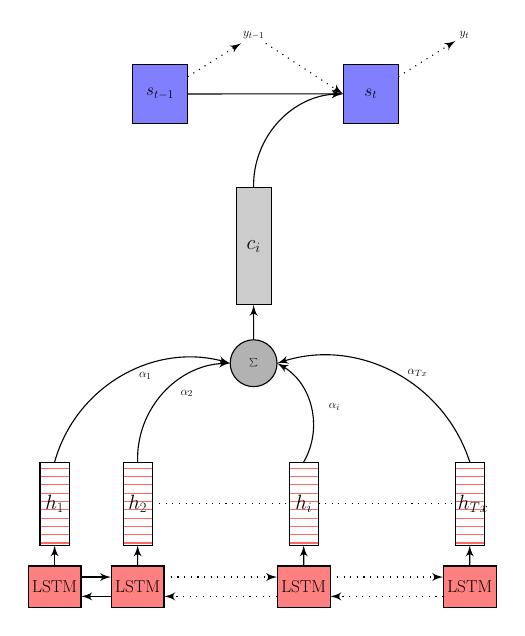
\begin{tikzpicture}[scale=0.3, every node/.style={transform shape}]
				\node[mlp_enc, node distance = 15em](LSTM_N_1){LSTM};
				\node[mlp_enc, right of=LSTM_N_1](LSTM_N_2) {LSTM};
				\path [line] (LSTM_N_1.20) to (LSTM_N_1.20-|LSTM_N_2.west);
				\path [line] (LSTM_N_2.200) to (LSTM_N_2.-20-|LSTM_N_1.east);     
				
				\node[mlp_enc, right of=LSTM_N_2, node distance = 20em](LSTM_N_i) {LSTM};
				\path [line, dotted] (LSTM_N_2.20) to (LSTM_N_2.20-|LSTM_N_i.west);
				\path [line, dotted] (LSTM_N_i.200) to (LSTM_N_i.200-|LSTM_N_2.east);
				
				\node[mlp_enc, right of=LSTM_N_i, node distance = 20em](LSTM_N_Tx) {LSTM};
				\path [line, dotted] (LSTM_N_i.20) to (LSTM_N_i.20-|LSTM_N_Tx.west);
				\path [line, dotted] (LSTM_N_Tx.200) to (LSTM_N_Tx.200-|LSTM_N_i.east);
				
				
				\node [enc_h, above of = LSTM_N_1] (h1) {$h_{1}$};
				\node [enc_h,above of = LSTM_N_2] (h2) {$h_{2}$};
				\node [enc_h,above of = LSTM_N_i] (hi) {$h_{i}$};
				\node [enc_h,above of = LSTM_N_Tx] (hTx) {$h_{Tx}$};

				\draw [dotted] (h2.east) to (hi.west);
				\draw [dotted] (hi.east) to (hTx.west);

				\path [line] (LSTM_N_1) to (h1);
				\path [line] (LSTM_N_2) to (h2);
				\path [line] (LSTM_N_i) to (hi);
				\path [line] (LSTM_N_Tx) to (hTx);
				
				
				\pause{}
				\fontsize{15}{12}
				\node [round, above of = h1, node distance = 12em, xshift=17em] (sum1) {$\sum$};
				
				\pause{}
				\path [line] (h1.north) to [bend left=45] node [xshift=2em] {$\alpha_{1}$} (sum1.west);
				\pause{}
				\path [line] (h2.north) to [bend left=45] node [xshift=2em] {$\alpha_{2}$} (sum1.west);
				\pause{}
				\path [line] (hi.north) to [bend right=45] node [xshift=2em] {$\alpha_{i}$} (sum1.east);
				\pause{}
				\path [line] (hTx.north) to [bend right=45] node [xshift=2em] {$\alpha_{Tx}$} (sum1.east);

				\pause{}
				\node [enc_h, above of = sum1, fill=black!20] (ci) {$c_{i}$};
				
				\path [line] (sum1) to (ci.south);
				
				\pause{}
				\node [mlp_dec, above of = ci, xshift = -8em, yshift = 3em] (decoder_tm1) {$s_{t-1}$};
				\node [above of = decoder_tm1, node distance = 5em, xshift = 8em] (ytm1) {$y_{t-1}$};
				\path [line, dotted] (decoder_tm1) to (ytm1);
				\pause{}
				\pause{}
				\node [mlp_dec, right of = decoder_tm1, xshift = 8em] (decoder_t) {$s_{t}$};
				\path [line] (decoder_tm1.east) to (decoder_t.west);
				\path [line] (ci.north) to [bend left=45] (decoder_t.west);
				\path [line, dotted] (ytm1) to (decoder_t.west);
				\pause{}
				\node [above of = decoder_t, node distance = 5em, xshift = 8em] (yt) {$y_{t}$};
				\path [line, dotted] (decoder_t) to (yt);
			\end{tikzpicture}
		\end{center}
	\end{frame}


	\section{No Attention [Equal Attention?]}
	
	
	\begin{frame}[fragile]{No Attention [Equal Attention?]}
	\begin{center}
	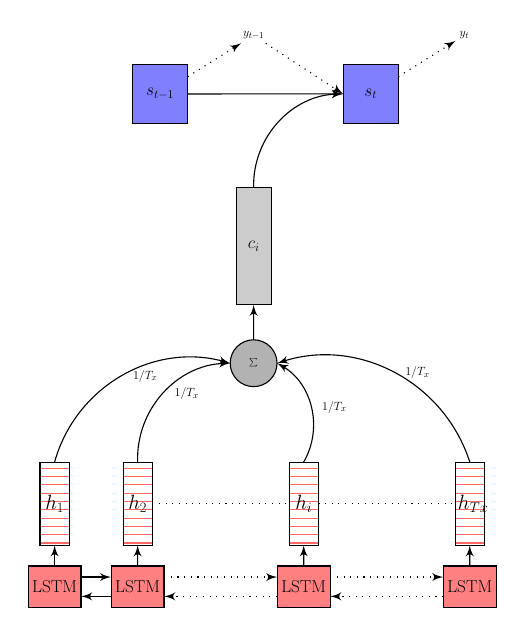
\begin{tikzpicture}[scale=0.3, every node/.style={transform shape}]
		\node[mlp_enc, node distance = 15em](LSTM_N_1){LSTM};
		\node[mlp_enc, right of=LSTM_N_1](LSTM_N_2) {LSTM};
		\path [line] (LSTM_N_1.20) to (LSTM_N_1.20-|LSTM_N_2.west);
		\path [line] (LSTM_N_2.200) to (LSTM_N_2.-20-|LSTM_N_1.east);     
		
		\node[mlp_enc, right of=LSTM_N_2, node distance = 20em](LSTM_N_i) {LSTM};
		\path [line, dotted] (LSTM_N_2.20) to (LSTM_N_2.20-|LSTM_N_i.west);
		\path [line, dotted] (LSTM_N_i.200) to (LSTM_N_i.200-|LSTM_N_2.east);
		
		\node[mlp_enc, right of=LSTM_N_i, node distance = 20em](LSTM_N_Tx) {LSTM};
		\path [line, dotted] (LSTM_N_i.20) to (LSTM_N_i.20-|LSTM_N_Tx.west);
		\path [line, dotted] (LSTM_N_Tx.200) to (LSTM_N_Tx.200-|LSTM_N_i.east);
		
		
		\node [enc_h, above of = LSTM_N_1] (h1) {$h_{1}$};
		\node [enc_h,above of = LSTM_N_2] (h2) {$h_{2}$};
		\node [enc_h,above of = LSTM_N_i] (hi) {$h_{i}$};
		\node [enc_h,above of = LSTM_N_Tx] (hTx) {$h_{Tx}$};
		
		\path [line] (LSTM_N_1) to (h1);
		\path [line] (LSTM_N_2) to (h2);
		\path [line] (LSTM_N_i) to (hi);
		\path [line] (LSTM_N_Tx) to (hTx);

		\draw [dotted] (h2.east) to (hi.west);
		\draw [dotted] (hi.east) to (hTx.west);
		
		
		\fontsize{15}{12}
		\node [round, above of = h1, node distance = 12em, xshift=17em] (sum1) {$\sum$};
		
		
		\path [line] (h1.north) to [bend left=45] node [xshift=2em] {$1/T_x$} (sum1.west);
		
		\path [line] (h2.north) to [bend left=45] node [xshift=2em] {$1/T_x$} (sum1.west);
		
		\path [line] (hi.north) to [bend right=45] node [xshift=2em] {$1/T_x$} (sum1.east);
		
		\path [line] (hTx.north) to [bend right=45] node [xshift=2em] {$1/T_x$} (sum1.east);
		
		
		\node [atts, above of = sum1, fill=black!20] (ci) {$c_{i}$};
		
		\path [line] (sum1) to (ci.south);
		
		
		\node [mlp_dec, above of = ci, xshift = -8em, yshift = 3em] (decoder_tm1) {$s_{t-1}$};
		\node [above of = decoder_tm1, node distance = 5em, xshift = 8em] (ytm1) {$y_{t-1}$};
		\path [line, dotted] (decoder_tm1) to (ytm1);
		
		
		\node [mlp_dec, right of = decoder_tm1, xshift = 8em] (decoder_t) {$s_{t}$};
		\path [line] (decoder_tm1.east) to (decoder_t.west);
		\path [line] (ci.north) to [bend left=45] (decoder_t.west);
		\path [line, dotted] (ytm1) to (decoder_t.west);
		
		\node [above of = decoder_t, node distance = 5em, xshift = 8em] (yt) {$y_{t}$};
		\path [line, dotted] (decoder_t) to (yt);
	\end{tikzpicture}
	\end{center}
	\end{frame}

	\begin{frame}[fragile]{Dimensions of representations}
	\begin{center}
		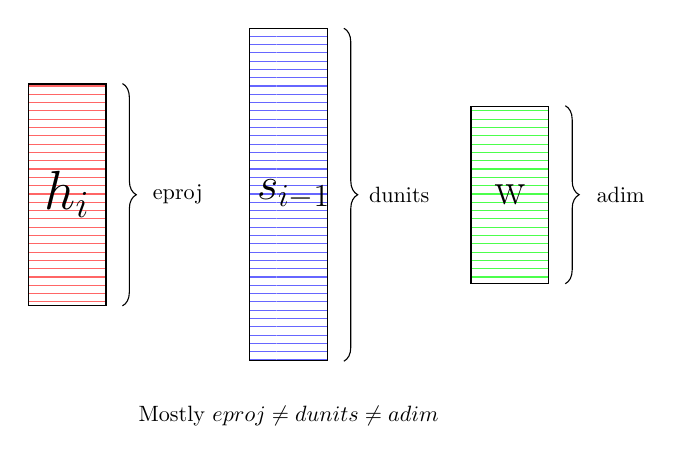
\begin{tikzpicture}[scale=0.8, every node/.style={transform shape}]
			\node [enc_h] (h1) {$h_{i}$};
			\draw [decorate,decoration={brace,amplitude=5pt, mirror, raise=2em}] (h1.south) -- (h1.north) node [black,midway,xshift=5em] {eproj};
			
			\node [dec_z, right of=h1, node distance = 10em, minimum height = 15em] (dec_z) {$s_{i-1}$};
			\draw [decorate,decoration={brace,amplitude=5pt, mirror, raise=2em}] (dec_z.south) -- (dec_z.north) node [black,midway,xshift=5em] {dunits};
			
			\node [atts, right of=dec_z, node distance = 10em, minimum height = 8em] (alpha) {w};
			\draw [decorate,decoration={brace,amplitude=5pt, mirror, raise=2em}] (alpha.south) -- (alpha.north) node [black,midway,xshift=5em] {adim};
			\node [below of=dec_z, node distance = 10em] {Mostly $ eproj \ne dunits \ne adim $};
		\end{tikzpicture}
	\end{center}
	\end{frame}

	\begin{frame}[fragile]{Matching the dimensions of representations}
	\begin{center}
		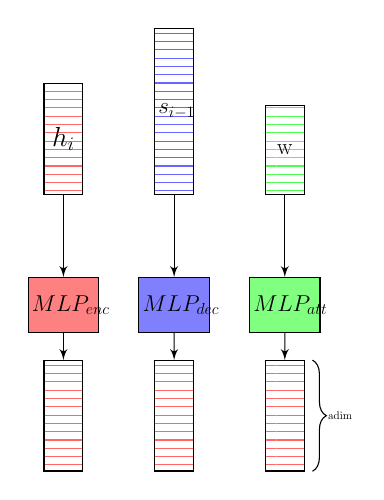
\begin{tikzpicture}[scale=0.4, every node/.style={transform shape}]
			\node [enc_h] (h1) {$h_{i}$};
		
			\node [dec_z, right of=h1, node distance = 10em, minimum height = 15em, yshift=2.5em] (dec_z) {$s_{i-1}$};
			
			\node [atts, right of=dec_z, node distance = 10em, minimum height = 8em, yshift=-3.5em] (alpha) {w};
			
			\node [mlp_enc, below of=h1, node distance = 15em] (mlp_enc) {$MLP_{enc}$};
			\node [mlp_dec, right of=mlp_enc, node distance = 10em] (mlp_dec) {$MLP_{dec}$};
			\node [mlp_att, right of=mlp_dec, node distance = 10em] (mlp_att) {$MLP_{att}$};
			
			\path [line] (h1.south) to (mlp_enc.north);
			\path [line] (dec_z.south) to (mlp_dec.north);
			\path [line] (alpha.south) to (mlp_att.north);
			
			\node [enc_h, below of=mlp_enc, node distance = 10em] (h_att) {};
			\node [enc_h, below of=mlp_dec, node distance = 10em] (z_att) {};
			\node [enc_h, below of=mlp_att, node distance = 10em] (alpha_att) {};
			
			\path [line] (mlp_enc.south) to (h_att.north);
			\path [line] (mlp_dec.south) to (z_att.north);
			\path [line] (mlp_att.south) to (alpha_att.north);
			\draw [decorate,decoration={brace,amplitude=5pt, mirror, raise=1em}] (alpha_att.south) -- (alpha_att.north) node [black,midway,xshift=5em] {adim};
		\end{tikzpicture}
	\end{center}
	\end{frame}
	
	
	\section{Dot product Attention}
	
	
	\begin{frame}[fragile]{Dot product Attention}
	\begin{center}
		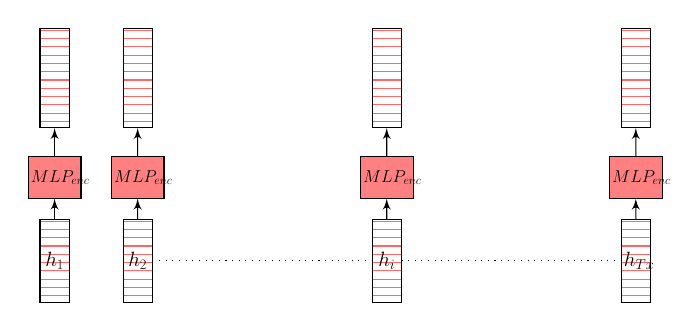
\begin{tikzpicture}[scale=0.3, every node/.style={transform shape}]
		\node [enc_h] (h1) {$h_{1}$};
		\node [enc_h,right of = h1] (h2) {$h_{2}$};
		\node [enc_h,right of = h2, node distance = 30em] (hi) {$h_{i}$};
		\node [enc_h,right of = hi, node distance = 30em] (hTx) {$h_{Tx}$};
		\draw [dotted] (h2.east) to (hi.west);
		\draw [dotted] (hi.east) to (hTx.west);
		\pause{}
		
		\node [mlp_enc, above of = h1, node distance = 10em] (mlp1) {$MLP_{enc}$};
		\path [line] (h1.north) to (mlp1.south);
		\node [enc_h, above of = mlp1, minimum height = 12em, node distance = 12em] (he1) {};
		\path [line] (mlp1.north) to (he1.south);
		
		\pause{}
		\node [mlp_enc, above of = h2, node distance = 10em] (mlp2) {$MLP_{enc}$};
		\path [line] (h2.north) to (mlp2.south);
		\node [enc_h, above of = mlp2, minimum height = 12em, node distance = 12em] (he2) {};
		\path [line] (mlp2.north) to (he2.south);
		
		\pause{}
		\node [mlp_enc, above of = hi, node distance = 10em] (mlpi) {$MLP_{enc}$};
		\path [line] (hi.north) to (mlpi.south);
		\node [enc_h, above of = mlpi, minimum height = 12em, node distance = 12em] (hei) {};
		\path [line] (mlpi.north) to (hei.south);
		
		\pause{}
		\node [mlp_enc, above of = hTx, node distance = 10em] (mlpTx) {$MLP_{enc}$};
		\path [line] (hTx.north) to (mlpTx.south);
		\node [enc_h, above of = mlpTx, minimum height = 12em, node distance = 12em] (heTx) {};
		\path [line] (mlpTx.north) to (heTx.south);
		\end{tikzpicture}
	\end{center}
\end{frame}

\begin{frame}[fragile]{Dot product Attention}
\begin{center}
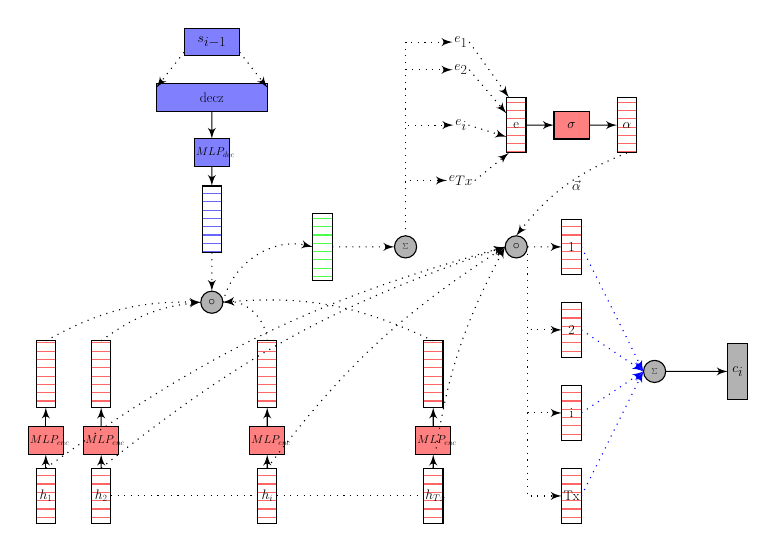
\begin{tikzpicture}[scale=0.2, every node/.style={transform shape}]
\node [enc_h] (h1) {$h_{1}$};
\node [enc_h,right of = h1] (h2) {$h_{2}$};
\node [enc_h,right of = h2, node distance = 30em] (hi) {$h_{i}$};
\node [enc_h,right of = hi, node distance = 30em] (hTx) {$h_{Tx}$};
\draw [dotted] (h2.east) to (hi.west);
\draw [dotted] (hi.east) to (hTx.west);


\node [mlp_enc, above of = h1, node distance = 10em] (mlp1) {$MLP_{enc}$};
\path [line] (h1.north) to (mlp1.south);
\node [enc_h, above of = mlp1, minimum height = 12em, node distance = 12em] (he1) {};
\path [line] (mlp1.north) to (he1.south);


\node [mlp_enc, above of = h2, node distance = 10em] (mlp2) {$MLP_{enc}$};
\path [line] (h2.north) to (mlp2.south);
\node [enc_h, above of = mlp2, minimum height = 12em, node distance = 12em] (he2) {};
\path [line] (mlp2.north) to (he2.south);


\node [mlp_enc, above of = hi, node distance = 10em] (mlpi) {$MLP_{enc}$};
\path [line] (hi.north) to (mlpi.south);
\node [enc_h, above of = mlpi, minimum height = 12em, node distance = 12em] (hei) {};
\path [line] (mlpi.north) to (hei.south);


\node [mlp_enc, above of = hTx, node distance = 10em] (mlpTx) {$MLP_{enc}$};
\path [line] (hTx.north) to (mlpTx.south);
\node [enc_h, above of = mlpTx, minimum height = 12em, node distance = 12em] (heTx) {};
\path [line] (mlpTx.north) to (heTx.south);

\node [mlp_dec, above of = hei, node distance = 60em, minimum width = 10em, xshift = -10em, font=\fontsize{40}{10}\selectfont] (sim1) {$s_{i-1}$};
\node [mlp_dec, below of=sim1, minimum width = 20em, font=\fontsize{40}{10}\selectfont] (dec_z) {decz};
\path [line, dotted] (sim1.200) to (dec_z.170);
\path [line, dotted] (sim1.-20) to (dec_z.10);
\node [mlp_dec, below of=dec_z, node distance = 10em] (mlp_dec) {$MLP_{dec}$};
\path [line] (dec_z) to (mlp_dec);
\node [dec_z, below of = mlp_dec, minimum height = 12em, node distance = 12em] (decz_enc) {};
\path [line] (mlp_dec) to (decz_enc);

\uncover<2-7>{
	\node [round, below of = decz_enc, node distance = 15em] (prod) {$\circ$}; 
	\path [line, dotted] (decz_enc.south) to (prod.north);
	\uncover<2-4>{
		\path [line, dotted] (he1.north) to [bend left=15] (prod.west);
	}
	\node [atts, right of = prod, minimum height = 12em, node distance = 20em, yshift=10em] (h_z) {};
	\path [line, dotted] (prod.east) to [bend left=45] (h_z.west);
}

\uncover<3-7>{
	\node [round, right of = h_z, node distance = 15em] (sum) {$\sum$};
	\path [line, dotted] (h_z.east) to (sum.west);
}

\uncover<4->{
	\node [right of=sim1, node distance = 15em, xshift=30em, font=\fontsize{40}{10}\selectfont] (e1) {$e_{1}$};
	\uncover<4>{
		\path [line, dotted] (sum.north) |- (e1.west);
	}
}

\uncover<5->{
	\node [below of=e1, node distance = 5em, font=\fontsize{40}{10}\selectfont] (e2) {$e_{2}$};
	\uncover<5>{
		\path [line, dotted] (he2.north) to [bend left=15] (prod.west);
		\path [line, dotted] (sum.north) |- (e2.west);
	}
}

\uncover<6->{
	\node [below of=e2, node distance = 10em, font=\fontsize{40}{10}\selectfont] (ei) {$e_{i}$};
	\uncover<6>{
		\path [line, dotted] (hei.north) to [bend right=45] (prod.east);
		\path [line, dotted] (sum.north) |- (ei.west);
	}
}

\uncover<7->{
	\node [below of=ei, node distance = 10em, font=\fontsize{40}{10}\selectfont] (eTx) {$e_{Tx}$};
	\only<7>{
		\path [line, dotted] (heTx.north) to [bend right=15] (prod.east);
		\path [line, dotted] (sum.north) |- (eTx.west);
	}
}

\uncover<8->{
	\node [enc_h, right of=ei, font=\fontsize{40}{10}\selectfont] (e) {e};
	
	
	\path [line, dotted] (e1.east) to (e.105);
	\path [line, dotted] (e2.east) to (e.130);
	\path [line, dotted] (ei.east) to (e.-130);
	\path [line, dotted] (eTx.east) to (e.-105);
	
	
	\node [mlp_enc, right of=e, font=\fontsize{40}{10}\selectfont] (sm) {$\sigma$};
	\path [line] (e.east) to (sm.west);
	
	
	\node [enc_h, right of=sm, font=\fontsize{40}{10}\selectfont] (alphas) {$\alpha$};
	\path [line] (sm.east) to (alphas.west);
}

\uncover<9>{
	\node [round, right of=sum, node distance=20em] (alpha_h) {$\circ$};
	\path [line, dotted, color=black] (h1.north) to [bend left=10] (alpha_h.west);
	\path [line, dotted, color=black] (alphas.south) to [bend right=15] node [xshift=2em] {\fontsize{40}{10}\selectfont $\vec{\alpha}$} (alpha_h.north);
	
	
	\node [enc_h, right of=alpha_h] (ahe1) {1};
	\path [line, dotted, color=black] (alpha_h.east) to (ahe1.west);
	
	\path [line, dotted, color=black] (h2.north) to [bend left=10] (alpha_h.west);
	\node [enc_h, below of=ahe1, node distance = 15em] (ahe2) {2};
	\path [line, dotted, color=black] (alpha_h.east) |- (ahe2.west);
	
	
	\path [line, dotted, color=black] (hi.north) to [bend left=10] (alpha_h.west);
	\node [enc_h, below of=ahe2, node distance = 15em] (ahei) {i};
	\path [line, dotted, color=black] (alpha_h.east) |- (ahei.west);
	
	\path [line, dotted, color=black] (hTx.north) to [bend left=10] (alpha_h.west);
	\node [enc_h, below of=ahei, node distance = 15em] (aheTx) {Tx};
	\path [line, dotted, color=black] (alpha_h.east) |- (aheTx.west);
	
	\pause{}
	\node [round, right of=ahe2, yshift=-7.5em, node distance = 15em] (sum_op) {$\sum$};
	\path [line, dotted, color=blue] (ahe1.east) to (sum_op.west);
	\path [line, dotted, color=blue] (ahe2.east) to (sum_op.west);
	\path [line, dotted, color=blue] (ahei.east) to (sum_op.west);
	\path [line, dotted, color=blue] (aheTx.east) to (sum_op.west);
	
	\pause{}
	\node [enc_h, right of=sum_op, fill=black!30, node distance=15em, font=\fontsize{40}{10}\selectfont] (ci) {$c_i$};
	\path [line] (sum_op.east) to (ci.west);
}
\end{tikzpicture}
\end{center}
\end{frame}


\begin{frame}[fragile]{Dot product Attention - Full picture}
\begin{center}
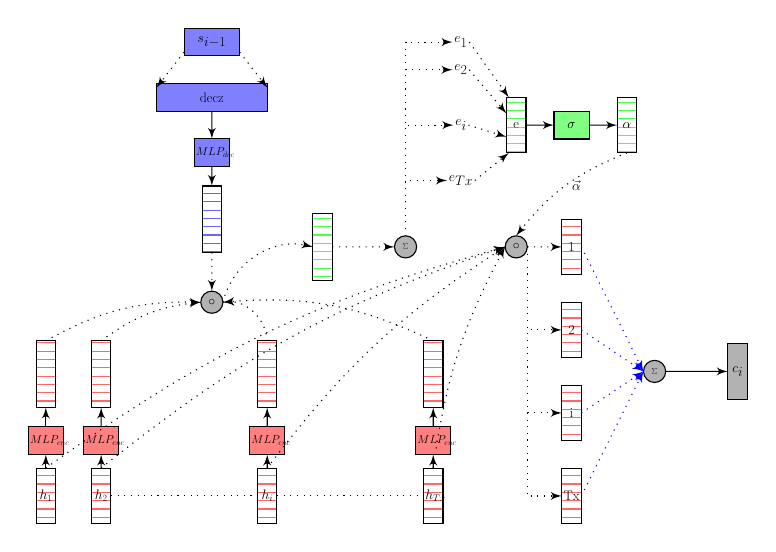
\begin{tikzpicture}[scale=0.2, every node/.style={transform shape}]
\node [enc_h] (h1) {$h_{1}$};
\node [enc_h,right of = h1] (h2) {$h_{2}$};
\node [enc_h,right of = h2, node distance = 30em] (hi) {$h_{i}$};
\node [enc_h,right of = hi, node distance = 30em] (hTx) {$h_{Tx}$};
\draw [dotted] (h2.east) to (hi.west);
\draw [dotted] (hi.east) to (hTx.west);


\node [mlp_enc, above of = h1, node distance = 10em] (mlp1) {$MLP_{enc}$};
\path [line] (h1.north) to (mlp1.south);
\node [enc_h, above of = mlp1, minimum height = 12em, node distance = 12em] (he1) {};
\path [line] (mlp1.north) to (he1.south);


\node [mlp_enc, above of = h2, node distance = 10em] (mlp2) {$MLP_{enc}$};
\path [line] (h2.north) to (mlp2.south);
\node [enc_h, above of = mlp2, minimum height = 12em, node distance = 12em] (he2) {};
\path [line] (mlp2.north) to (he2.south);


\node [mlp_enc, above of = hi, node distance = 10em] (mlpi) {$MLP_{enc}$};
\path [line] (hi.north) to (mlpi.south);
\node [enc_h, above of = mlpi, minimum height = 12em, node distance = 12em] (hei) {};
\path [line] (mlpi.north) to (hei.south);


\node [mlp_enc, above of = hTx, node distance = 10em] (mlpTx) {$MLP_{enc}$};
\path [line] (hTx.north) to (mlpTx.south);
\node [enc_h, above of = mlpTx, minimum height = 12em, node distance = 12em] (heTx) {};
\path [line] (mlpTx.north) to (heTx.south);

\node [mlp_dec, above of = hei, node distance = 60em, minimum width = 10em, xshift = -10em, font=\fontsize{40}{10}\selectfont] (sim1) {$s_{i-1}$};
\node [mlp_dec, below of=sim1, minimum width = 20em, font=\fontsize{40}{10}\selectfont] (dec_z) {decz};
\path [line, dotted] (sim1.200) to (dec_z.170);
\path [line, dotted] (sim1.-20) to (dec_z.10);
\node [mlp_dec, below of=dec_z, node distance = 10em] (mlp_dec) {$MLP_{dec}$};
\path [line] (dec_z) to (mlp_dec);
\node [dec_z, below of = mlp_dec, minimum height = 12em, node distance = 12em] (decz_enc) {};
\path [line] (mlp_dec) to (decz_enc);


\node [round, below of = decz_enc, node distance = 15em] (prod) {$\circ$}; 
\path [line, dotted] (decz_enc.south) to (prod.north);

\path [line, dotted] (he1.north) to [bend left=15] (prod.west);
\node [atts, right of = prod, minimum height = 12em, node distance = 20em, yshift=10em] (h_z) {};
\path [line, dotted] (prod.east) to [bend left=45] (h_z.west);


\node [round, right of = h_z, node distance = 15em] (sum) {$\sum$};
\path [line, dotted] (h_z.east) to (sum.west);



\node [right of=sim1, node distance = 15em, xshift=30em, font=\fontsize{40}{10}\selectfont] (e1) {$e_{1}$};

\path [line, dotted] (sum.north) |- (e1.west);

\node [below of=e1, node distance = 5em, font=\fontsize{40}{10}\selectfont] (e2) {$e_{2}$};

\path [line, dotted] (he2.north) to [bend left=15] (prod.west);
\path [line, dotted] (sum.north) |- (e2.west);



\node [below of=e2, node distance = 10em, font=\fontsize{40}{10}\selectfont] (ei) {$e_{i}$};

\path [line, dotted] (hei.north) to [bend right=45] (prod.east);
\path [line, dotted] (sum.north) |- (ei.west);



\node [below of=ei, node distance = 10em, font=\fontsize{40}{10}\selectfont] (eTx) {$e_{Tx}$};

\path [line, dotted] (heTx.north) to [bend right=15] (prod.east);
\path [line, dotted] (sum.north) |- (eTx.west);


\node [atts, right of=ei, font=\fontsize{40}{10}\selectfont] (e) {e};


\path [line, dotted] (e1.east) to (e.105);
\path [line, dotted] (e2.east) to (e.130);
\path [line, dotted] (ei.east) to (e.-130);
\path [line, dotted] (eTx.east) to (e.-105);


\node [mlp_att, right of=e, font=\fontsize{40}{10}\selectfont] (sm) {$\sigma$};
\path [line] (e.east) to (sm.west);


\node [atts, right of=sm, font=\fontsize{40}{10}\selectfont] (alphas) {$\alpha$};
\path [line] (sm.east) to (alphas.west);


\node [round, right of=sum, node distance=20em] (alpha_h) {$\circ$};
\path [line, dotted, color=black] (h1.north) to [bend left=10] (alpha_h.west);
\path [line, dotted, color=black] (alphas.south) to [bend right=15] node [xshift=2em] {\fontsize{40}{10}\selectfont $\vec{\alpha}$} (alpha_h.north);


\node [enc_h, right of=alpha_h] (ahe1) {1};
\path [line, dotted, color=black] (alpha_h.east) to (ahe1.west);

\path [line, dotted, color=black] (h2.north) to [bend left=10] (alpha_h.west);
\node [enc_h, below of=ahe1, node distance = 15em] (ahe2) {2};
\path [line, dotted, color=black] (alpha_h.east) |- (ahe2.west);


\path [line, dotted, color=black] (hi.north) to [bend left=10] (alpha_h.west);
\node [enc_h, below of=ahe2, node distance = 15em] (ahei) {i};
\path [line, dotted, color=black] (alpha_h.east) |- (ahei.west);

\path [line, dotted, color=black] (hTx.north) to [bend left=10] (alpha_h.west);
\node [enc_h, below of=ahei, node distance = 15em] (aheTx) {Tx};
\path [line, dotted, color=black] (alpha_h.east) |- (aheTx.west);

\node [round, right of=ahe2, yshift=-7.5em, node distance = 15em] (sum_op) {$\sum$};
\path [line, dotted, color=blue] (ahe1.east) to (sum_op.west);
\path [line, dotted, color=blue] (ahe2.east) to (sum_op.west);
\path [line, dotted, color=blue] (ahei.east) to (sum_op.west);
\path [line, dotted, color=blue] (aheTx.east) to (sum_op.west);


\node [enc_h, right of=sum_op, fill=black!30, node distance=15em, font=\fontsize{40}{10}\selectfont] (ci) {$c_i$};
\path [line] (sum_op.east) to (ci.west);
\end{tikzpicture}
\end{center}
\end{frame}


	
	\section{Additive Attention}
	

	\begin{frame}[fragile]{Additive Attention}
	\begin{center}
		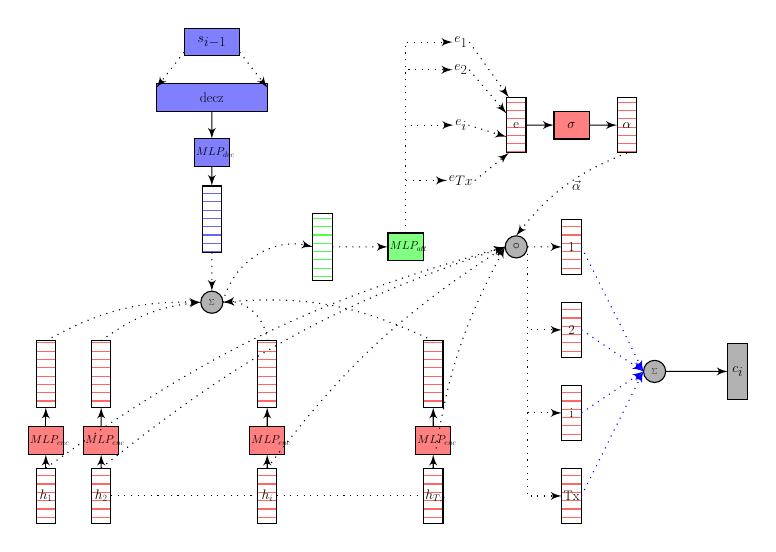
\begin{tikzpicture}[scale=0.2, every node/.style={transform shape}]
		\node [enc_h] (h1) {$h_{1}$};
		\node [enc_h,right of = h1] (h2) {$h_{2}$};
		\node [enc_h,right of = h2, node distance = 30em] (hi) {$h_{i}$};
		\node [enc_h,right of = hi, node distance = 30em] (hTx) {$h_{Tx}$};
		\draw [dotted] (h2.east) to (hi.west);
		\draw [dotted] (hi.east) to (hTx.west);
		
		
		\node [mlp_enc, above of = h1, node distance = 10em] (mlp1) {$MLP_{enc}$};
		\path [line] (h1.north) to (mlp1.south);
		\node [enc_h, above of = mlp1, minimum height = 12em, node distance = 12em] (he1) {};
		\path [line] (mlp1.north) to (he1.south);
		
		
		\node [mlp_enc, above of = h2, node distance = 10em] (mlp2) {$MLP_{enc}$};
		\path [line] (h2.north) to (mlp2.south);
		\node [enc_h, above of = mlp2, minimum height = 12em, node distance = 12em] (he2) {};
		\path [line] (mlp2.north) to (he2.south);
		
		
		\node [mlp_enc, above of = hi, node distance = 10em] (mlpi) {$MLP_{enc}$};
		\path [line] (hi.north) to (mlpi.south);
		\node [enc_h, above of = mlpi, minimum height = 12em, node distance = 12em] (hei) {};
		\path [line] (mlpi.north) to (hei.south);
		
		
		\node [mlp_enc, above of = hTx, node distance = 10em] (mlpTx) {$MLP_{enc}$};
		\path [line] (hTx.north) to (mlpTx.south);
		\node [enc_h, above of = mlpTx, minimum height = 12em, node distance = 12em] (heTx) {};
		\path [line] (mlpTx.north) to (heTx.south);
		
		\node [mlp_dec, above of = hei, node distance = 60em, minimum width = 10em, xshift = -10em, font=\fontsize{40}{10}\selectfont] (sim1) {$s_{i-1}$};
		\node [mlp_dec, below of=sim1, minimum width = 20em, font=\fontsize{40}{10}\selectfont] (dec_z) {decz};
		\path [line, dotted] (sim1.200) to (dec_z.170);
		\path [line, dotted] (sim1.-20) to (dec_z.10);
		\node [mlp_dec, below of=dec_z, node distance = 10em] (mlp_dec) {$MLP_{dec}$};
		\path [line] (dec_z) to (mlp_dec);
		\node [dec_z, below of = mlp_dec, minimum height = 12em, node distance = 12em] (decz_enc) {};
		\path [line] (mlp_dec) to (decz_enc);
		
		\uncover<2-7>{
			\node [round, below of = decz_enc, node distance = 15em] (prod) {$\sum$}; 
			\path [line, dotted] (decz_enc.south) to (prod.north);
			\uncover<2-4>{
				\path [line, dotted] (he1.north) to [bend left=15] (prod.west);
			}
			\node [atts, right of = prod, minimum height = 12em, node distance = 20em, yshift=10em] (h_z) {};
			\path [line, dotted] (prod.east) to [bend left=45] (h_z.west);
		}
		
		\uncover<3-7>{
			\node [mlp_att, right of = h_z, node distance = 15em] (sum) {$MLP_{att}$};
			%		\node [round, right of = h_z, node distance = 15em] (sum) {$\sum$};
			\path [line, dotted] (h_z.east) to (sum.west);
		}
		
		\uncover<4->{
			\node [right of=sim1, node distance = 15em, xshift=30em, font=\fontsize{40}{10}\selectfont] (e1) {$e_{1}$};
			\uncover<4>{
				\path [line, dotted] (sum.north) |- (e1.west);
			}
		}
		
		\uncover<5->{
			\node [below of=e1, node distance = 5em, font=\fontsize{40}{10}\selectfont] (e2) {$e_{2}$};
			\uncover<5>{
				\path [line, dotted] (he2.north) to [bend left=15] (prod.west);
				\path [line, dotted] (sum.north) |- (e2.west);
			}
		}
		
		\uncover<6->{
			\node [below of=e2, node distance = 10em, font=\fontsize{40}{10}\selectfont] (ei) {$e_{i}$};
			\uncover<6>{
				\path [line, dotted] (hei.north) to [bend right=45] (prod.east);
				\path [line, dotted] (sum.north) |- (ei.west);
			}
		}
		
		\uncover<7->{
			\node [below of=ei, node distance = 10em, font=\fontsize{40}{10}\selectfont] (eTx) {$e_{Tx}$};
			\only<7>{
				\path [line, dotted] (heTx.north) to [bend right=15] (prod.east);
				\path [line, dotted] (sum.north) |- (eTx.west);
			}
		}
		
		\uncover<8->{
			\node [enc_h, right of=ei, font=\fontsize{40}{10}\selectfont] (e) {e};
			
			
			\path [line, dotted] (e1.east) to (e.105);
			\path [line, dotted] (e2.east) to (e.130);
			\path [line, dotted] (ei.east) to (e.-130);
			\path [line, dotted] (eTx.east) to (e.-105);
			
			
			\node [mlp_enc, right of=e, font=\fontsize{40}{10}\selectfont] (sm) {$\sigma$};
			\path [line] (e.east) to (sm.west);
			
			
			\node [enc_h, right of=sm, font=\fontsize{40}{10}\selectfont] (alphas) {$\alpha$};
			\path [line] (sm.east) to (alphas.west);
		}
		\uncover<9>{
			\node [round, right of=sum, node distance=20em] (alpha_h) {$\circ$};
			\path [line, dotted, color=black] (h1.north) to [bend left=10] (alpha_h.west);
			\path [line, dotted, color=black] (alphas.south) to [bend right=15] node [xshift=2em] {\fontsize{40}{10}\selectfont $\vec{\alpha}$} (alpha_h.north);
			
			
			\node [enc_h, right of=alpha_h] (ahe1) {1};
			\path [line, dotted, color=black] (alpha_h.east) to (ahe1.west);
			
			\path [line, dotted, color=black] (h2.north) to [bend left=10] (alpha_h.west);
			\node [enc_h, below of=ahe1, node distance = 15em] (ahe2) {2};
			\path [line, dotted, color=black] (alpha_h.east) |- (ahe2.west);
			
			
			\path [line, dotted, color=black] (hi.north) to [bend left=10] (alpha_h.west);
			\node [enc_h, below of=ahe2, node distance = 15em] (ahei) {i};
			\path [line, dotted, color=black] (alpha_h.east) |- (ahei.west);
			
			\path [line, dotted, color=black] (hTx.north) to [bend left=10] (alpha_h.west);
			\node [enc_h, below of=ahei, node distance = 15em] (aheTx) {Tx};
			\path [line, dotted, color=black] (alpha_h.east) |- (aheTx.west);
			
			\pause{}
			\node [round, right of=ahe2, yshift=-7.5em, node distance = 15em] (sum_op) {$\sum$};
			\path [line, dotted, color=blue] (ahe1.east) to (sum_op.west);
			\path [line, dotted, color=blue] (ahe2.east) to (sum_op.west);
			\path [line, dotted, color=blue] (ahei.east) to (sum_op.west);
			\path [line, dotted, color=blue] (aheTx.east) to (sum_op.west);
			
			\pause{}
			\node [enc_h, right of=sum_op, fill=black!30, node distance=15em, font=\fontsize{40}{10}\selectfont] (ci) {$c_i$};
			\path [line] (sum_op.east) to (ci.west);
		}
		\end{tikzpicture}
	\end{center}
\end{frame}


\begin{frame}[fragile]{Additive Attention - Full picture}
\begin{center}
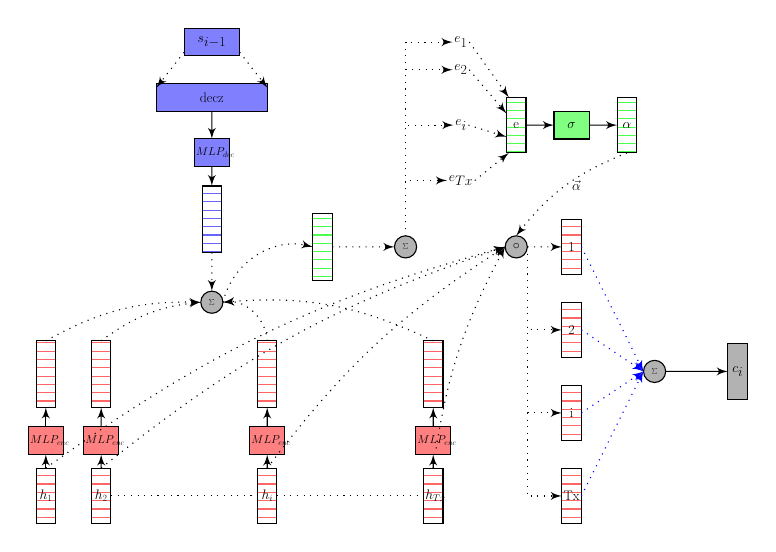
\begin{tikzpicture}[scale=0.2, every node/.style={transform shape}]
\node [enc_h] (h1) {$h_{1}$};
\node [enc_h,right of = h1] (h2) {$h_{2}$};
\node [enc_h,right of = h2, node distance = 30em] (hi) {$h_{i}$};
\node [enc_h,right of = hi, node distance = 30em] (hTx) {$h_{Tx}$};
\draw [dotted] (h2.east) to (hi.west);
\draw [dotted] (hi.east) to (hTx.west);


\node [mlp_enc, above of = h1, node distance = 10em] (mlp1) {$MLP_{enc}$};
\path [line] (h1.north) to (mlp1.south);
\node [enc_h, above of = mlp1, minimum height = 12em, node distance = 12em] (he1) {};
\path [line] (mlp1.north) to (he1.south);


\node [mlp_enc, above of = h2, node distance = 10em] (mlp2) {$MLP_{enc}$};
\path [line] (h2.north) to (mlp2.south);
\node [enc_h, above of = mlp2, minimum height = 12em, node distance = 12em] (he2) {};
\path [line] (mlp2.north) to (he2.south);


\node [mlp_enc, above of = hi, node distance = 10em] (mlpi) {$MLP_{enc}$};
\path [line] (hi.north) to (mlpi.south);
\node [enc_h, above of = mlpi, minimum height = 12em, node distance = 12em] (hei) {};
\path [line] (mlpi.north) to (hei.south);


\node [mlp_enc, above of = hTx, node distance = 10em] (mlpTx) {$MLP_{enc}$};
\path [line] (hTx.north) to (mlpTx.south);
\node [enc_h, above of = mlpTx, minimum height = 12em, node distance = 12em] (heTx) {};
\path [line] (mlpTx.north) to (heTx.south);

\node [mlp_dec, above of = hei, node distance = 60em, minimum width = 10em, xshift = -10em, font=\fontsize{40}{10}\selectfont] (sim1) {$s_{i-1}$};
\node [mlp_dec, below of=sim1, minimum width = 20em, font=\fontsize{40}{10}\selectfont] (dec_z) {decz};
\path [line, dotted] (sim1.200) to (dec_z.170);
\path [line, dotted] (sim1.-20) to (dec_z.10);
\node [mlp_dec, below of=dec_z, node distance = 10em] (mlp_dec) {$MLP_{dec}$};
\path [line] (dec_z) to (mlp_dec);
\node [dec_z, below of = mlp_dec, minimum height = 12em, node distance = 12em] (decz_enc) {};
\path [line] (mlp_dec) to (decz_enc);


\node [round, below of = decz_enc, node distance = 15em] (prod) {$\sum$}; 
\path [line, dotted] (decz_enc.south) to (prod.north);

\path [line, dotted] (he1.north) to [bend left=15] (prod.west);
\node [atts, right of = prod, minimum height = 12em, node distance = 20em, yshift=10em] (h_z) {};
\path [line, dotted] (prod.east) to [bend left=45] (h_z.west);


\node [round, right of = h_z, node distance = 15em] (sum) {$\sum$};
\path [line, dotted] (h_z.east) to (sum.west);



\node [right of=sim1, node distance = 15em, xshift=30em, font=\fontsize{40}{10}\selectfont] (e1) {$e_{1}$};

\path [line, dotted] (sum.north) |- (e1.west);

\node [below of=e1, node distance = 5em, font=\fontsize{40}{10}\selectfont] (e2) {$e_{2}$};

\path [line, dotted] (he2.north) to [bend left=15] (prod.west);
\path [line, dotted] (sum.north) |- (e2.west);



\node [below of=e2, node distance = 10em, font=\fontsize{40}{10}\selectfont] (ei) {$e_{i}$};

\path [line, dotted] (hei.north) to [bend right=45] (prod.east);
\path [line, dotted] (sum.north) |- (ei.west);



\node [below of=ei, node distance = 10em, font=\fontsize{40}{10}\selectfont] (eTx) {$e_{Tx}$};

\path [line, dotted] (heTx.north) to [bend right=15] (prod.east);
\path [line, dotted] (sum.north) |- (eTx.west);


\node [atts, right of=ei, font=\fontsize{40}{10}\selectfont] (e) {e};


\path [line, dotted] (e1.east) to (e.105);
\path [line, dotted] (e2.east) to (e.130);
\path [line, dotted] (ei.east) to (e.-130);
\path [line, dotted] (eTx.east) to (e.-105);


\node [mlp_att, right of=e, font=\fontsize{40}{10}\selectfont] (sm) {$\sigma$};
\path [line] (e.east) to (sm.west);


\node [atts, right of=sm, font=\fontsize{40}{10}\selectfont] (alphas) {$\alpha$};
\path [line] (sm.east) to (alphas.west);


\node [round, right of=sum, node distance=20em] (alpha_h) {$\circ$};
\path [line, dotted, color=black] (h1.north) to [bend left=10] (alpha_h.west);
\path [line, dotted, color=black] (alphas.south) to [bend right=15] node [xshift=2em] {\fontsize{40}{10}\selectfont $\vec{\alpha}$} (alpha_h.north);


\node [enc_h, right of=alpha_h] (ahe1) {1};
\path [line, dotted, color=black] (alpha_h.east) to (ahe1.west);

\path [line, dotted, color=black] (h2.north) to [bend left=10] (alpha_h.west);
\node [enc_h, below of=ahe1, node distance = 15em] (ahe2) {2};
\path [line, dotted, color=black] (alpha_h.east) |- (ahe2.west);


\path [line, dotted, color=black] (hi.north) to [bend left=10] (alpha_h.west);
\node [enc_h, below of=ahe2, node distance = 15em] (ahei) {i};
\path [line, dotted, color=black] (alpha_h.east) |- (ahei.west);

\path [line, dotted, color=black] (hTx.north) to [bend left=10] (alpha_h.west);
\node [enc_h, below of=ahei, node distance = 15em] (aheTx) {Tx};
\path [line, dotted, color=black] (alpha_h.east) |- (aheTx.west);

\node [round, right of=ahe2, yshift=-7.5em, node distance = 15em] (sum_op) {$\sum$};
\path [line, dotted, color=blue] (ahe1.east) to (sum_op.west);
\path [line, dotted, color=blue] (ahe2.east) to (sum_op.west);
\path [line, dotted, color=blue] (ahei.east) to (sum_op.west);
\path [line, dotted, color=blue] (aheTx.east) to (sum_op.west);


\node [enc_h, right of=sum_op, fill=black!30, node distance=15em, font=\fontsize{40}{10}\selectfont] (ci) {$c_i$};
\path [line] (sum_op.east) to (ci.west);
\end{tikzpicture}
\end{center}
\end{frame}



	\section{Location Aware Attention}
	
	\begin{frame}[fragile]{Location Aware Attention}
	\begin{center}
		\begin{tikzpicture}[scale=0.7, every node/.style={transform shape}]
		\only<1>{
			\node [draw, rectangle] (alpha_t) {$\alpha_{1}^{t-1}$ \hspace{1em} $\alpha_{2}^{t-1}$ \dots \dots \dots $\alpha_{i}^{t-1}$ \dots \dots \dots $\alpha_{Tx}^{t-1}$};
			\node [draw, rectangle, above of = alpha_t, node distance = 2em] (alpha_t_padded) {0 \hspace{1em} 0 \dots \hspace{1em} 0  $\alpha_{1}^{t-1}$ \hspace{1em} $\alpha_{2}^{t-1}$ \dots \dots \dots $\alpha_{i}^{t-1}$ \dots \dots \dots $\alpha_{Tx}^{t-1}$ 0 \hspace{1em} 0 \dots \hspace{1em} 0};
			\node [above of = alpha_t_padded, node distance = 2em] (conv) {*};
			
			\node [draw, rectangle, above of = alpha_t_padded, node distance = 4em, fill=blue!10] (w1)
			{$w_{1}^{1}$ $w_{2}^{1}$ \dots $w_{i}^{1}$ \dots $w_{filt\_size}^{1}$};
			\begin{scope}[on background layer]
			\node [draw, rectangle, above of = w1, node distance = 1.5em, fill=blue!10, xshift=1em] (w2)
			{$w_{1}^{2}$ $w_{2}^{2}$ \dots $w_{i}^{2}$ \dots $w_{filt\_size}^{2}$};
			\end{scope}
			
			\node [draw, rectangle, above of = w2, node distance = 4em, fill=blue!10, xshift=4em] (wT)
			{$w_{1}^{nf}$ $w_{2}^{nf}$ \dots $w_{i}^{nf}$ \dots $w_{filt\_size}^{nf}$};
			\path [line, dotted] (w2.171) to (wT.171);
			\path [line, dotted] (w2.9) to (wT.9);	
		}
		
		\only<2-3>{
			\node [draw, rectangle, above of = alpha_t, node distance = 2em] (alpha_t_padded) {0 \hspace{1em} 0 \dots \hspace{1em} 0  $\alpha_{1}^{t-1}$ \hspace{1em} $\alpha_{2}^{t-1}$ \dots \dots \dots $\alpha_{i}^{t-1}$ \dots \dots \dots $\alpha_{Tx}^{t-1}$ 0 \hspace{1em} 0 \dots \hspace{1em} 0};
			\node [above of = alpha_t_padded, node distance = 2em] (conv) {*};
			
			\only<2>{
				\node [draw, rectangle, above of = alpha_t_padded, node distance = 4em, fill=blue!10] (w1)
				{$w_{1}^{1}$ $w_{2}^{1}$ \dots $w_{i}^{1}$ \dots $w_{filt\_size}^{1}$};
				\node [above of = w1, yshift=-5] (eq1) {\rotatebox{90}{$\,=$}};
				\node [draw, rectangle, above of = w1, node distance = 4em, fill=green!50] (w1)
				{$\beta_{1}^{1}$ \hspace{1em} $\beta_{2}^{1}$ \dots  \dots \dots $\beta_{i}^{1}$ \dots \dots \dots $\beta_{Tx}^{1}$};
			}
			\only<3>{
				\node [draw, rectangle, above of = alpha_t_padded, node distance = 4em, fill=blue!10] (w2)
				{$w_{1}^{2}$ $w_{2}^{2}$ \dots $w_{i}^{2}$ \dots $w_{filt\_size}^{2}$};
				\node [above of = w2, yshift=-5] (eq1) {\rotatebox{90}{$\,=$}};
				\node [draw, rectangle, above of = w2, node distance = 4em, fill=green!50] (w1)
				{$\beta_{1}^{2}$ \hspace{1em} $\beta_{2}^{2}$ \dots  \dots \dots $\beta_{i}^{2}$ \dots \dots \dots $\beta_{Tx}^{2}$};
			}
		}
		
		
		\only<4>{
			\node [draw, rectangle] (alpha_t) {$\alpha_{1}^{t-1}$ \hspace{1em} $\alpha_{2}^{t-1}$ \dots \dots \dots $\alpha_{i}^{t-1}$ \dots \dots \dots $\alpha_{Tx}^{t-1}$};
			\node [draw, rectangle, above of = alpha_t, node distance = 2em] (alpha_t_padded) {0 \hspace{1em} 0 \dots \hspace{1em} 0  $\alpha_{1}^{t-1}$ \hspace{1em} $\alpha_{2}^{t-1}$ \dots \dots \dots $\alpha_{i}^{t-1}$ \dots \dots \dots $\alpha_{Tx}^{t-1}$ 0 \hspace{1em} 0 \dots \hspace{1em} 0};
			\node [above of = alpha_t_padded, node distance = 2em] (conv) {*};
			
			\node [draw, rectangle, above of = alpha_t_padded, node distance = 4em, fill=blue!10] (w1)
			{$w_{1}^{1}$ $w_{2}^{1}$ \dots $w_{i}^{1}$ \dots $w_{filt\_size}^{1}$};
			\begin{scope}[on background layer]
			\node [draw, rectangle, above of = w1, node distance = 1.5em, fill=blue!10, xshift=1em] (w2)
			{$w_{1}^{2}$ $w_{2}^{2}$ \dots $w_{i}^{2}$ \dots $w_{filt\_size}^{2}$};
			\end{scope}
			
			\node [draw, rectangle, above of = w2, node distance = 4em, fill=blue!10, xshift=4em] (wT)
			{$w_{1}^{nf}$ $w_{2}^{nf}$ \dots $w_{i}^{nf}$ \dots $w_{filt\_size}^{nf}$};
			\path [line, dotted] (w2.171) to (wT.171);
			\path [line, dotted] (w2.9) to (wT.9);	
			
			\node [above of = wT, yshift=-5] (eq1) {\rotatebox{45}{$\,=$}};
			
			\node [atts, above of = wT, pattern=crosshatch, node distance = 10em] (b1) {$\beta_{1}^{1}$ \newline . \newline . \newline . \newline $\beta_{1}^{10}$} ;
			\node [atts, right of = b1, pattern=crosshatch, node distance = 10em] (b2) {$\beta_{Tx}^{1}$ \newline . \newline . \newline . \newline $\beta_{Tx}^{10}$} ;
			\path [line, densely dotted, -] (b1.east) to (b2.west);
			
			\draw [decorate,decoration={brace,amplitude=5pt, raise=0.5em}] (b1.north) -- (b2.north) node [black,midway, yshift=2em] {Tx};
		}
		\end{tikzpicture}
	\end{center}
\end{frame}

\begin{frame}[fragile]{Location Aware Attention - Full picture}
\begin{center}
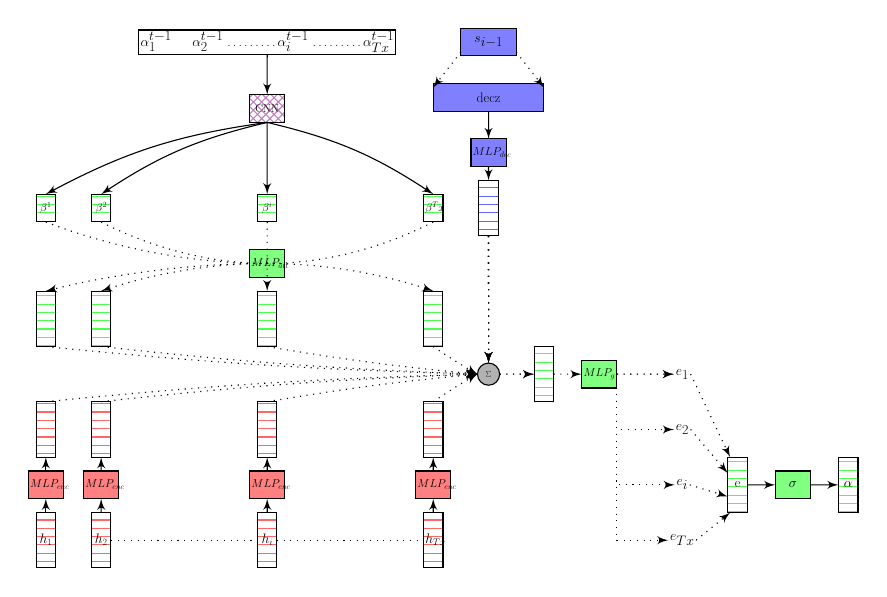
\begin{tikzpicture}[scale=0.2, every node/.style={transform shape}]
\node [enc_h] (h1) {$h_{1}$};
\node [enc_h,right of = h1] (h2) {$h_{2}$};
\node [enc_h,right of = h2, node distance = 30em] (hi) {$h_{i}$};
\node [enc_h,right of = hi, node distance = 30em] (hTx) {$h_{Tx}$};
\draw [dotted] (h2.east) to (hi.west);
\draw [dotted] (hi.east) to (hTx.west);


\node [mlp_enc, above of = h1, node distance = 10em] (mlp1) {$MLP_{enc}$};
\path [line] (h1.north) to (mlp1.south);
\node [enc_h, above of = mlp1] (he1) {};
\path [line] (mlp1.north) to (he1.south);


\node [mlp_enc, above of = h2, node distance = 10em] (mlp2) {$MLP_{enc}$};
\path [line] (h2.north) to (mlp2.south);
\node [enc_h, above of = mlp2] (he2) {};
\path [line] (mlp2.north) to (he2.south);


\node [mlp_enc, above of = hi, node distance = 10em] (mlpi) {$MLP_{enc}$};
\path [line] (hi.north) to (mlpi.south);
\node [enc_h, above of = mlpi] (hei) {};
\path [line] (mlpi.north) to (hei.south);


\node [mlp_enc, above of = hTx, node distance = 10em] (mlpTx) {$MLP_{enc}$};
\path [line] (hTx.north) to (mlpTx.south);
\node [enc_h, above of = mlpTx] (heTx) {};
\path [line] (mlpTx.north) to (heTx.south);
\node [draw, rectangle, above of=hei, node distance = 70em,font=\fontsize{40}{10}\selectfont] (alpha_t) {$\alpha_{1}^{t-1}$ \hspace{1em} $\alpha_{2}^{t-1}$ \dots \dots \dots $\alpha_{i}^{t-1}$ \dots \dots \dots $\alpha_{Tx}^{t-1}$};
\node [cnn, below of=alpha_t, node distance = 12em] (cnn1) {CNN};
\path [line] (alpha_t.south) to (cnn1.north);
\node [atts, above of = he1,minimum height=5em, node distance = 40em] (beta1) {$\beta^1$};
\node [atts, above of = he2, minimum height=5em, node distance = 40em] (beta2) {$\beta^2$};
\node [atts, above of = hei, minimum height=5em, node distance = 40em] (betai) {$\beta^i$};
\node [atts, above of = heTx, minimum height=5em, node distance = 40em] (betaTx) {$\beta^Tx$};

\path [line] (cnn1.south) to [bend right=10] (beta1.north);
\path [line] (cnn1.south) to [bend right=10] (beta2.north);
\path [line] (cnn1.south) to (betai.north);
\path [line] (cnn1.south) to [bend left=10] (betaTx.north);

\node [mlp_att, below of=betai, node distance = 10em] (mlpatt) {$MLP_{att}$};
\node [atts, below of = beta1, node distance = 20em] (beta1_enc) {};
\node [atts, below of = beta2, node distance = 20em] (beta2_enc) {};
\node [atts, below of = betai, node distance = 20em] (betai_enc) {};
\node [atts, below of = betaTx, node distance = 20em] (betaTx_enc) {};
\path [line, dotted] (beta1.south) parabola bend (mlpatt) (beta1_enc.north);
\path [line, dotted] (beta2.south) parabola bend (mlpatt) (beta2_enc.north);
\path [line, dotted] (betai.south) parabola bend (mlpatt) (betai_enc.north);
\path [line, dotted] (betaTx.south) parabola bend (mlpatt) (betaTx_enc.north);

\node [round, below of=betaTx_enc, node distance=10em, xshift=10em] (sum1) {$\sum$};

\node [mlp_dec, right of = betaTx, node distance = 10em, minimum width = 10em, yshift=30em, font=\fontsize{40}{10}\selectfont] (sim1) {$s_{i-1}$};
\node [mlp_dec, below of=sim1, minimum width = 20em, font=\fontsize{40}{10}\selectfont] (dec_z) {decz};
\path [line, dotted] (sim1.200) to (dec_z.170);
\path [line, dotted] (sim1.-20) to (dec_z.10);
\node [mlp_dec, below of=dec_z, node distance = 10em] (mlp_dec) {$MLP_{dec}$};
\path [line] (dec_z) to (mlp_dec);
\node [dec_z, below of = mlp_dec] (decz_enc) {};
\path [line] (mlp_dec) to (decz_enc);

\path [line, dotted] (beta1_enc.south) to [bend right=2] (sum1.west);
\path [line, dotted] (he1.north) to [bend left=2] (sum1.west);
\path [line, dotted] (decz_enc.south) to (sum1.north);

\path [line, dotted] (beta2_enc.south) to [bend right=2] (sum1.west);
\path [line, dotted] (he2.north) to [bend left=2] (sum1.west);
\path [line, dotted] (decz_enc.south) to (sum1.north);

\path [line, dotted] (betai_enc.south) to [bend right=2] (sum1.west);
\path [line, dotted] (hei.north) to [bend left=2] (sum1.west);
\path [line, dotted] (decz_enc.south) to (sum1.north);

\path [line, dotted] (betaTx_enc.south) to [bend right=2] (sum1.west);
\path [line, dotted] (heTx.north) to [bend left=2] (sum1.west);
\path [line, dotted] (decz_enc.south) to (sum1.north);

\node [atts, right of=sum1, node distance = 10em] (asdf) {};
\node [mlp_att, right of=asdf] (mlpg) {$MLP_{g}$};
\node [right of=mlpg, node distance=15em, font=\fontsize{40}{10}\selectfont] (e1) {$e_1$};

\node [below of=e1, node distance=10em, font=\fontsize{40}{10}\selectfont] (e2) {$e_2$};

\node [below of=e2, node distance=10em, font=\fontsize{40}{10}\selectfont] (ei) {$e_i$};

\node [below of=ei, node distance=10em, font=\fontsize{40}{10}\selectfont] (eTx) {$e_{Tx}$};

\node [atts, right of=ei, font=\fontsize{40}{10}\selectfont] (e) {e};

\path [line, dotted] (e1.east) to (e.105);
\path [line, dotted] (e2.east) to (e.130);
\path [line, dotted] (ei.east) to (e.-130);
\path [line, dotted] (eTx.east) to (e.-105);

\node [mlp_att, right of=e, font=\fontsize{40}{10}\selectfont] (sm) {$\sigma$};
\path [line] (e.east) to (sm.west);


\node [atts, right of=sm, font=\fontsize{40}{10}\selectfont] (alphas) {$\alpha$};
\path [line] (sm.east) to (alphas.west);

\path [line, dotted] (sum1.east) to (asdf.west);
\path [line, dotted] (sum1.east) to (asdf.west);
\path [line, dotted] (asdf.east) to (mlpg.west);
\path [line, dotted] (mlpg.east) to (e1.west);
\path [line, dotted] (mlpg.east) to (e1.west);
\path [line, dotted] (mlpg.east) |- (e2.west);
\path [line, dotted] (mlpg.east) |- (ei.west);
\path [line, dotted] (mlpg.east) |- (eTx.west);


\end{tikzpicture}
\end{center}
\end{frame}



	\section{2D Location Aware Attention}
	\begin{frame}[fragile]{2D Location Aware Attention}
	\begin{center}
		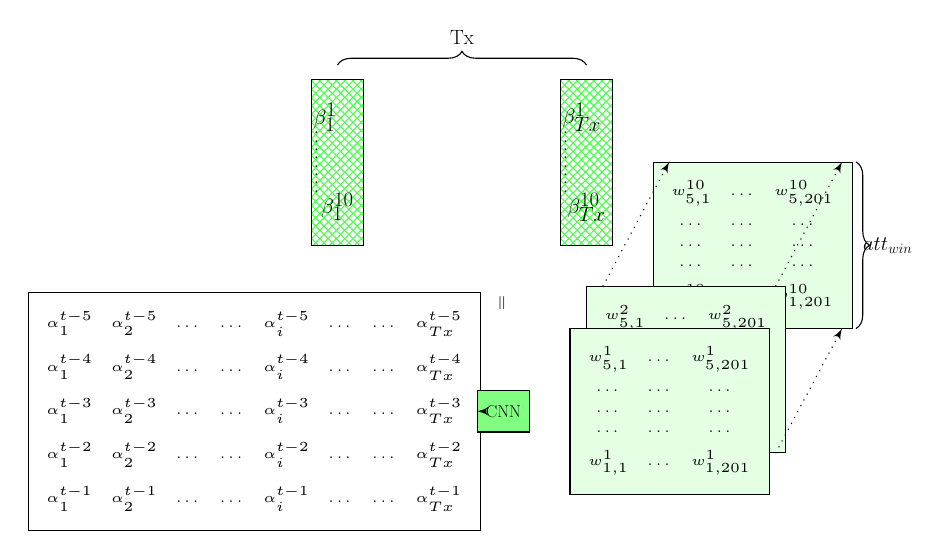
\begin{tikzpicture}[scale=0.3, every node/.style={transform shape, font=\fontsize{5}{10}\selectfont}]
		\matrix [matrix of nodes, draw, .style={nodes={draw=none, minimum width=1em}}] (m)
		{
			$\alpha_{1}^{t-5}$ & $\alpha_{2}^{t-5}$ & \dots  & \dots & $\alpha_{i}^{t-5}$ & \dots & \dots & $\alpha_{Tx}^{t-5}$ \\
			
			$\alpha_{1}^{t-4}$ & $\alpha_{2}^{t-4}$ & \dots  & \dots & $\alpha_{i}^{t-4}$ & \dots & \dots & $\alpha_{Tx}^{t-4}$ \\
			
			$\alpha_{1}^{t-3}$ & $\alpha_{2}^{t-3}$ & \dots  & \dots & $\alpha_{i}^{t-3}$ & \dots & \dots & $\alpha_{Tx}^{t-3}$ \\
			
			$\alpha_{1}^{t-2}$ & $\alpha_{2}^{t-2}$ & \dots  & \dots & $\alpha_{i}^{t-2}$ & \dots & \dots & $\alpha_{Tx}^{t-2}$ \\
			
			$\alpha_{1}^{t-1}$ & $\alpha_{2}^{t-1}$ & \dots  & \dots & $\alpha_{i}^{t-1}$ & \dots & \dots & $\alpha_{Tx}^{t-1}$ \\
		};
		
		\node [mlp_att, right of=m, node distance = 30em] (cnn1) {CNN};
		\path [line] (m.east) to (cnn1.west);
		\matrix [matrix of nodes, right of = cnn1,fill=green!10, node distance = 20em, draw, .style={nodes={draw=none, minimum width=1em}}] (m1)
		{
			$w_{5,1}^{1}$ & \dots & $w_{5,201}^{1}$ \\
			
			\dots & \dots & \dots \\
			
			\dots & \dots & \dots \\
			
			\dots & \dots & \dots \\
			
			$w_{1,1}^{1}$ & \dots & $w_{1,201}^{1}$ \\
		};
		
		\begin{scope}[on background layer]
		\matrix [matrix of nodes, above of = m1, fill=green!10, xshift=10em, node distance = 20em, draw, .style={nodes={draw=none, minimum width=1em}}] (m3)
		{
			$w_{5,1}^{10}$ & \dots & $w_{5,201}^{10}$ \\
			
			\dots & \dots & \dots \\
			
			\dots & \dots & \dots \\
			
			\dots & \dots & \dots \\
			
			$w_{1,1}^{10}$ & \dots & $w_{1,201}^{10}$ \\
		};
		\end{scope}
		
		\begin{scope}[on background layer]
		\matrix [matrix of nodes, above of = m1, fill=green!10, xshift=2em, node distance = 5em, draw, .style={nodes={draw=none, minimum width=1em}}] (m2)
		{
			$w_{5,1}^{2}$ & \dots & $w_{5,201}^{2}$ \\
			
			\dots & \dots & \dots \\
			
			\dots & \dots & \dots \\
			
			\dots & \dots & \dots \\
			
			$w_{1,1}^{2}$ & \dots & $w_{1,201}^{2}$ \\
		};
		\end{scope}
		
		
		\draw [decorate,decoration={brace,amplitude=5pt, raise=0.5em}] (m3.43) -- (m3.-43) node [black,midway, xshift=5.5em] {\fontsize{25}{10}\selectfont $att_{win}$};
		
		\path [line, dotted] (m2.135) to (m3.135);
		\path [line, dotted] (m2.43) to (m3.43);
		\path [line, dotted] (m2.-43) to (m3.-43);
		
		\node [atts, above of = cnn1, pattern=crosshatch, node distance = 30em, minimum height = 20em, text width=2cm,font=\fontsize{40}{10}\selectfont, xshift=-20em] (b1) {$\beta_{1}^{1}$ \newline . \newline . \newline . \newline . \newline . \newline . \newline . \newline . \newline $\beta_{1}^{10}$} ;
		
		\node [atts, right of = b1, pattern=crosshatch, node distance = 30em, minimum height = 20em, text width=2cm,font=\fontsize{40}{10}\selectfont] (b2) {$\beta_{Tx}^{1}$ \newline . \newline . \newline . \newline . \newline . \newline . \newline . \newline . \newline $\beta_{Tx}^{10}$} ;
		
		\draw [decorate,decoration={brace,amplitude=5pt, raise=0.5em}] (b1.north) -- (b2.north) node [black,midway, yshift=5em] {\fontsize{40}{10}\selectfont Tx};
		
		\node [above of = cnn1, yshift=10em, font=\fontsize{40}{10}\selectfont] (eq1) {\rotatebox{90}{$\,=$}};
		\end{tikzpicture}
	\end{center}
\end{frame}


\begin{frame}[fragile]{2D Location Aware Attention - Full picture}
\begin{center}
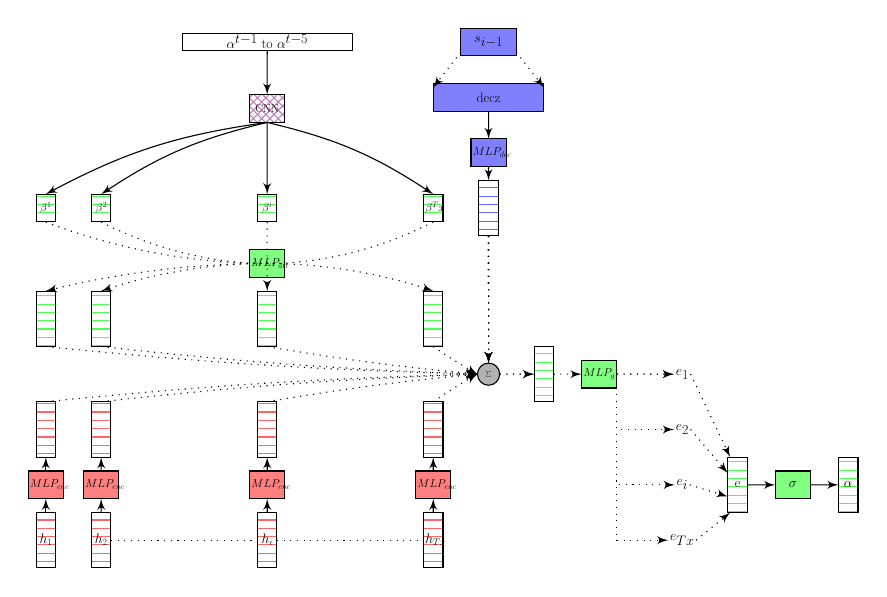
\begin{tikzpicture}[scale=0.2, every node/.style={transform shape}]
\node [enc_h] (h1) {$h_{1}$};
\node [enc_h,right of = h1] (h2) {$h_{2}$};
\node [enc_h,right of = h2, node distance = 30em] (hi) {$h_{i}$};
\node [enc_h,right of = hi, node distance = 30em] (hTx) {$h_{Tx}$};
\draw [dotted] (h2.east) to (hi.west);
\draw [dotted] (hi.east) to (hTx.west);


\node [mlp_enc, above of = h1, node distance = 10em] (mlp1) {$MLP_{enc}$};
\path [line] (h1.north) to (mlp1.south);
\node [enc_h, above of = mlp1] (he1) {};
\path [line] (mlp1.north) to (he1.south);


\node [mlp_enc, above of = h2, node distance = 10em] (mlp2) {$MLP_{enc}$};
\path [line] (h2.north) to (mlp2.south);
\node [enc_h, above of = mlp2] (he2) {};
\path [line] (mlp2.north) to (he2.south);


\node [mlp_enc, above of = hi, node distance = 10em] (mlpi) {$MLP_{enc}$};
\path [line] (hi.north) to (mlpi.south);
\node [enc_h, above of = mlpi] (hei) {};
\path [line] (mlpi.north) to (hei.south);


\node [mlp_enc, above of = hTx, node distance = 10em] (mlpTx) {$MLP_{enc}$};
\path [line] (hTx.north) to (mlpTx.south);
\node [enc_h, above of = mlpTx] (heTx) {};
\path [line] (mlpTx.north) to (heTx.south);

\node [draw, rectangle, above of=hei, node distance = 70em,font=\fontsize{40}{10}\selectfont, text width = 30em, text centered] (alpha_t) {$\alpha^{t-1}$ to $\alpha^{t-5}$};

\node [cnn, below of=alpha_t, node distance = 12em] (cnn1) {CNN};
\path [line] (alpha_t.south) to (cnn1.north);
\node [atts, above of = he1,minimum height=5em, node distance = 40em] (beta1) {$\beta^1$};
\node [atts, above of = he2, minimum height=5em, node distance = 40em] (beta2) {$\beta^2$};
\node [atts, above of = hei, minimum height=5em, node distance = 40em] (betai) {$\beta^i$};
\node [atts, above of = heTx, minimum height=5em, node distance = 40em] (betaTx) {$\beta^Tx$};

\path [line] (cnn1.south) to [bend right=10] (beta1.north);
\path [line] (cnn1.south) to [bend right=10] (beta2.north);
\path [line] (cnn1.south) to (betai.north);
\path [line] (cnn1.south) to [bend left=10] (betaTx.north);

\node [mlp_att, below of=betai, node distance = 10em] (mlpatt) {$MLP_{att}$};
\node [atts, below of = beta1, node distance = 20em] (beta1_enc) {};
\node [atts, below of = beta2, node distance = 20em] (beta2_enc) {};
\node [atts, below of = betai, node distance = 20em] (betai_enc) {};
\node [atts, below of = betaTx, node distance = 20em] (betaTx_enc) {};
\path [line, dotted] (beta1.south) parabola bend (mlpatt) (beta1_enc.north);
\path [line, dotted] (beta2.south) parabola bend (mlpatt) (beta2_enc.north);
\path [line, dotted] (betai.south) parabola bend (mlpatt) (betai_enc.north);
\path [line, dotted] (betaTx.south) parabola bend (mlpatt) (betaTx_enc.north);

\node [round, below of=betaTx_enc, node distance=10em, xshift=10em] (sum1) {$\sum$};

\node [mlp_dec, right of = betaTx, node distance = 10em, minimum width = 10em, yshift=30em, font=\fontsize{40}{10}\selectfont] (sim1) {$s_{i-1}$};
\node [mlp_dec, below of=sim1, minimum width = 20em, font=\fontsize{40}{10}\selectfont] (dec_z) {decz};
\path [line, dotted] (sim1.200) to (dec_z.170);
\path [line, dotted] (sim1.-20) to (dec_z.10);
\node [mlp_dec, below of=dec_z, node distance = 10em] (mlp_dec) {$MLP_{dec}$};
\path [line] (dec_z) to (mlp_dec);
\node [dec_z, below of = mlp_dec] (decz_enc) {};
\path [line] (mlp_dec) to (decz_enc);

\path [line, dotted] (beta1_enc.south) to [bend right=2] (sum1.west);
\path [line, dotted] (he1.north) to [bend left=2] (sum1.west);
\path [line, dotted] (decz_enc.south) to (sum1.north);

\path [line, dotted] (beta2_enc.south) to [bend right=2] (sum1.west);
\path [line, dotted] (he2.north) to [bend left=2] (sum1.west);
\path [line, dotted] (decz_enc.south) to (sum1.north);

\path [line, dotted] (betai_enc.south) to [bend right=2] (sum1.west);
\path [line, dotted] (hei.north) to [bend left=2] (sum1.west);
\path [line, dotted] (decz_enc.south) to (sum1.north);

\path [line, dotted] (betaTx_enc.south) to [bend right=2] (sum1.west);
\path [line, dotted] (heTx.north) to [bend left=2] (sum1.west);
\path [line, dotted] (decz_enc.south) to (sum1.north);

\node [atts, right of=sum1, node distance = 10em] (asdf) {};
\node [mlp_att, right of=asdf] (mlpg) {$MLP_{g}$};
\node [right of=mlpg, node distance=15em, font=\fontsize{40}{10}\selectfont] (e1) {$e_1$};

\node [below of=e1, node distance=10em, font=\fontsize{40}{10}\selectfont] (e2) {$e_2$};

\node [below of=e2, node distance=10em, font=\fontsize{40}{10}\selectfont] (ei) {$e_i$};

\node [below of=ei, node distance=10em, font=\fontsize{40}{10}\selectfont] (eTx) {$e_{Tx}$};

\node [atts, right of=ei, font=\fontsize{40}{10}\selectfont] (e) {e};

\path [line, dotted] (e1.east) to (e.105);
\path [line, dotted] (e2.east) to (e.130);
\path [line, dotted] (ei.east) to (e.-130);
\path [line, dotted] (eTx.east) to (e.-105);

\node [mlp_att, right of=e, font=\fontsize{40}{10}\selectfont] (sm) {$\sigma$};
\path [line] (e.east) to (sm.west);


\node [atts, right of=sm, font=\fontsize{40}{10}\selectfont] (alphas) {$\alpha$};
\path [line] (sm.east) to (alphas.west);

\path [line, dotted] (sum1.east) to (asdf.west);
\path [line, dotted] (sum1.east) to (asdf.west);
\path [line, dotted] (asdf.east) to (mlpg.west);
\path [line, dotted] (mlpg.east) to (e1.west);
\path [line, dotted] (mlpg.east) to (e1.west);
\path [line, dotted] (mlpg.east) |- (e2.west);
\path [line, dotted] (mlpg.east) |- (ei.west);
\path [line, dotted] (mlpg.east) |- (eTx.west);


\end{tikzpicture}
\end{center}
\end{frame}



\section{Location Aware Recurrent Attention}
\begin{frame}[fragile]{Location Aware Recurrent Attention}
\begin{center}
	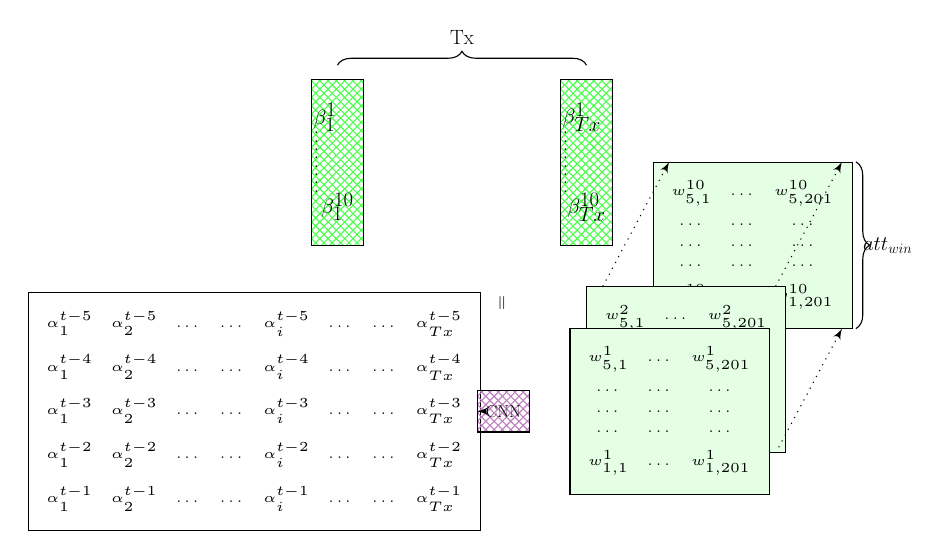
\begin{tikzpicture}[scale=0.3, every node/.style={transform shape, font=\fontsize{5}{10}\selectfont}]
	\matrix [matrix of nodes, draw, .style={nodes={draw=none, minimum width=1em}}] (m)
	{
		$\alpha_{1}^{t-5}$ & $\alpha_{2}^{t-5}$ & \dots  & \dots & $\alpha_{i}^{t-5}$ & \dots & \dots & $\alpha_{Tx}^{t-5}$ \\
		
		$\alpha_{1}^{t-4}$ & $\alpha_{2}^{t-4}$ & \dots  & \dots & $\alpha_{i}^{t-4}$ & \dots & \dots & $\alpha_{Tx}^{t-4}$ \\
		
		$\alpha_{1}^{t-3}$ & $\alpha_{2}^{t-3}$ & \dots  & \dots & $\alpha_{i}^{t-3}$ & \dots & \dots & $\alpha_{Tx}^{t-3}$ \\
		
		$\alpha_{1}^{t-2}$ & $\alpha_{2}^{t-2}$ & \dots  & \dots & $\alpha_{i}^{t-2}$ & \dots & \dots & $\alpha_{Tx}^{t-2}$ \\
		
		$\alpha_{1}^{t-1}$ & $\alpha_{2}^{t-1}$ & \dots  & \dots & $\alpha_{i}^{t-1}$ & \dots & \dots & $\alpha_{Tx}^{t-1}$ \\
	};
	
	\node [cnn, right of=m, node distance = 30em] (cnn1) {CNN};
	\path [line] (m.east) to (cnn1.west);
	\matrix [matrix of nodes, right of = cnn1,fill=green!10, node distance = 20em, draw, .style={nodes={draw=none, minimum width=1em}}] (m1)
	{
		$w_{5,1}^{1}$ & \dots & $w_{5,201}^{1}$ \\
		
		\dots & \dots & \dots \\
		
		\dots & \dots & \dots \\
		
		\dots & \dots & \dots \\
		
		$w_{1,1}^{1}$ & \dots & $w_{1,201}^{1}$ \\
	};
	
	\begin{scope}[on background layer]
	\matrix [matrix of nodes, above of = m1, fill=green!10, xshift=10em, node distance = 20em, draw, .style={nodes={draw=none, minimum width=1em}}] (m3)
	{
		$w_{5,1}^{10}$ & \dots & $w_{5,201}^{10}$ \\
		
		\dots & \dots & \dots \\
		
		\dots & \dots & \dots \\
		
		\dots & \dots & \dots \\
		
		$w_{1,1}^{10}$ & \dots & $w_{1,201}^{10}$ \\
	};
	\end{scope}
	
	\begin{scope}[on background layer]
	\matrix [matrix of nodes, above of = m1, fill=green!10, xshift=2em, node distance = 5em, draw, .style={nodes={draw=none, minimum width=1em}}] (m2)
	{
		$w_{5,1}^{2}$ & \dots & $w_{5,201}^{2}$ \\
		
		\dots & \dots & \dots \\
		
		\dots & \dots & \dots \\
		
		\dots & \dots & \dots \\
		
		$w_{1,1}^{2}$ & \dots & $w_{1,201}^{2}$ \\
	};
	\end{scope}
	
	
	\draw [decorate,decoration={brace,amplitude=5pt, raise=0.5em}] (m3.43) -- (m3.-43) node [black,midway, xshift=5.5em] {\fontsize{25}{10}\selectfont $att_{win}$};
	
	\path [line, dotted] (m2.135) to (m3.135);
	\path [line, dotted] (m2.43) to (m3.43);
	\path [line, dotted] (m2.-43) to (m3.-43);
	
	\node [atts, above of = cnn1, pattern=crosshatch, node distance = 30em, minimum height = 20em, text width=2cm,font=\fontsize{40}{10}\selectfont, xshift=-20em] (b1) {$\beta_{1}^{1}$ \newline . \newline . \newline . \newline . \newline . \newline . \newline . \newline . \newline $\beta_{1}^{10}$} ;
	
	\node [atts, right of = b1, pattern=crosshatch, node distance = 30em, minimum height = 20em, text width=2cm,font=\fontsize{40}{10}\selectfont] (b2) {$\beta_{Tx}^{1}$ \newline . \newline . \newline . \newline . \newline . \newline . \newline . \newline . \newline $\beta_{Tx}^{10}$} ;
	
	\draw [decorate,decoration={brace,amplitude=5pt, raise=0.5em}] (b1.north) -- (b2.north) node [black,midway, yshift=5em] {\fontsize{40}{10}\selectfont Tx};
	
	\node [above of = cnn1, yshift=10em, font=\fontsize{40}{10}\selectfont] (eq1) {\rotatebox{90}{$\,=$}};
	\end{tikzpicture}
\end{center}
\end{frame}

\begin{frame}[fragile]{Location Aware Recurrent Attention - weights}
\begin{center}
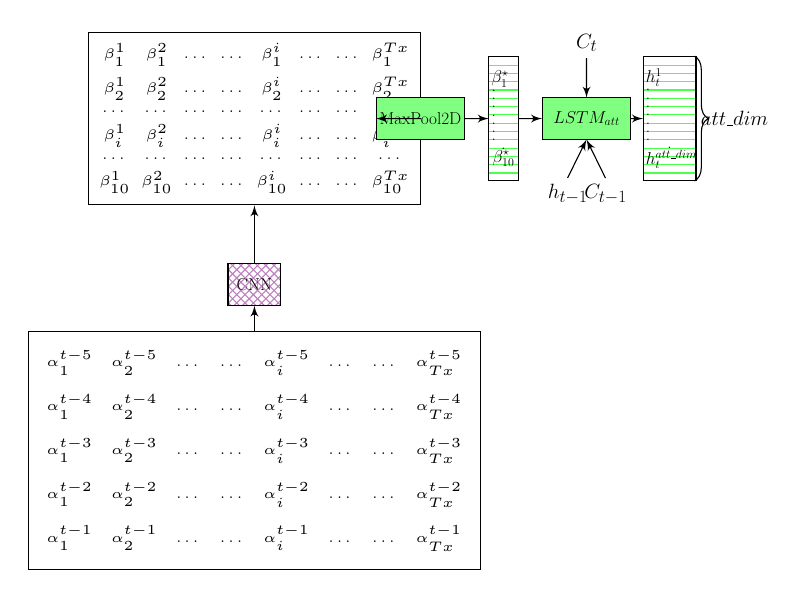
\begin{tikzpicture}[scale = 0.3, every node/.style={transform shape}]
\matrix [matrix of nodes, draw, .style={nodes={draw=none, minimum width=1em}}, font=\fontsize{4}{2}\selectfont] (m1)
{
	$\alpha_{1}^{t-5}$ & $\alpha_{2}^{t-5}$ & \dots  & \dots & $\alpha_{i}^{t-5}$ & \dots & \dots & $\alpha_{Tx}^{t-5}$ \\
	
	$\alpha_{1}^{t-4}$ & $\alpha_{2}^{t-4}$ & \dots  & \dots & $\alpha_{i}^{t-4}$ & \dots & \dots & $\alpha_{Tx}^{t-4}$ \\
	
	$\alpha_{1}^{t-3}$ & $\alpha_{2}^{t-3}$ & \dots  & \dots & $\alpha_{i}^{t-3}$ & \dots & \dots & $\alpha_{Tx}^{t-3}$ \\
	
	$\alpha_{1}^{t-2}$ & $\alpha_{2}^{t-2}$ & \dots  & \dots & $\alpha_{i}^{t-2}$ & \dots & \dots & $\alpha_{Tx}^{t-2}$ \\
	
	$\alpha_{1}^{t-1}$ & $\alpha_{2}^{t-1}$ & \dots  & \dots & $\alpha_{i}^{t-1}$ & \dots & \dots & $\alpha_{Tx}^{t-1}$ \\
};

\node [cnn, above of = m1, node distance = 20em] (cnn2) {CNN};
\path [line] (m1.north) to (cnn2.south);
\matrix [matrix of nodes, draw, above of = m1, node distance = 40em, .style={nodes={draw=none, minimum width=1em}}, font=\fontsize{3}{3}\selectfont, inner sep = 2pt] (m)
{
	$\beta_{1}^{1}$ & $\beta_{1}^{2}$ & \dots  & \dots & $\beta_{1}^{i}$ & \dots & \dots & $\beta_{1}^{Tx}$ \\
	
	$\beta_{2}^{1}$ & $\beta_{2}^{2}$ & \dots  & \dots & $\beta_{2}^{i}$ & \dots & \dots & $\beta_{2}^{Tx}$ \\
	
	\dots & \dots & \dots  & \dots & \dots & \dots & \dots & \dots \\
	
	$\beta_{i}^{1}$ & $\beta_{i}^{2}$ & \dots  & \dots & $\beta_{i}^{i}$ & \dots & \dots & $\beta_{i}^{Tx}$ \\
	
	\dots & \dots & \dots  & \dots & \dots & \dots & \dots & \dots \\
	
	$\beta_{10}^{1}$ & $\beta_{10}^{2}$ & \dots  & \dots & $\beta_{10}^{i}$ & \dots & \dots & $\beta_{10}^{Tx}$ \\
};
\path [line] (cnn2.north) to (m.south);
\node [mlp_att, right of = m, node distance = 20em, text width = 10em] (maxp) {MaxPool2D};

\path [line] (m.east) to (maxp.west);
\node [atts, right of = maxp, minimum height = 15em] (betastar) {$\beta_{1}^{\star}$ \newline . \newline . \newline . \newline . \newline . \newline . \newline . \newline . $\beta_{10}^{\star}$};

\path [line] (maxp.east) to (betastar.west);

\node [mlp_att, right of=betastar, text width = 10em] (lstm) {$LSTM_{att}$};

\path [line] (betastar.east) to (lstm.west);

\node [atts, right of=lstm, text width = 2cm, minimum height = 15em] (ht) {$h_{t}^{1}$ \newline . \newline . \newline . \newline . \newline . \newline . \newline . \newline . $h_{t}^{att\_dim}$};

\path [line] (lstm.east) to (ht.west);
{font=\fontsize{30}{30}\selectfont
	\node [below of=lstm, node distance = 4em, xshift=-1em] (htm1) {$h_{t-1}$};
	\node [below of=lstm, node distance = 4em, xshift=1em] (ctm1) {$C_{t-1}$};
	\node [above of=lstm, node distance = 4em] (ct) {$C_{t}$};
}
\path [line] (htm1.north) to (lstm.south);
\path [line] (ct.south) to (lstm.north);
\path [line] (ctm1.north) to (lstm.south);

\draw [decorate,decoration={brace,amplitude=5pt, raise=0.5em}] (ht.80) -- (ht.-80) node [black,midway, xshift=6.5em] {\fontsize{25}{10}\selectfont $att\_dim$};

\end{tikzpicture}
\end{center}
\end{frame}

\begin{frame}[fragile]{Location Aware Recurrent Attention - Full picture}
\begin{center}
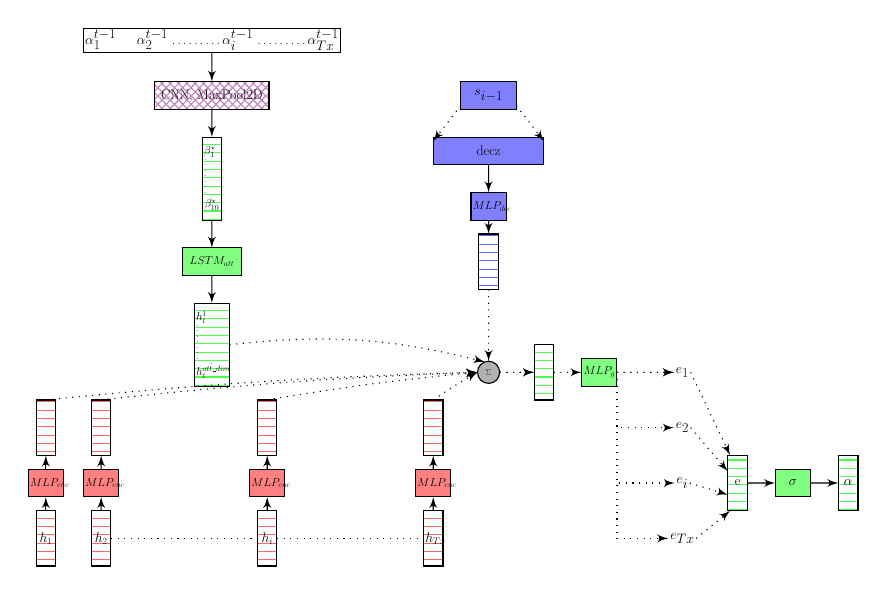
\begin{tikzpicture}[scale=0.2, every node/.style={transform shape}]
\node [enc_h] (h1) {$h_{1}$};
\node [enc_h,right of = h1] (h2) {$h_{2}$};
\node [enc_h,right of = h2, node distance = 30em] (hi) {$h_{i}$};
\node [enc_h,right of = hi, node distance = 30em] (hTx) {$h_{Tx}$};
\draw [dotted] (h2.east) to (hi.west);
\draw [dotted] (hi.east) to (hTx.west);


\node [mlp_enc, above of = h1, node distance = 10em] (mlp1) {$MLP_{enc}$};
\path [line] (h1.north) to (mlp1.south);
\node [enc_h, above of = mlp1] (he1) {};
\path [line] (mlp1.north) to (he1.south);


\node [mlp_enc, above of = h2, node distance = 10em] (mlp2) {$MLP_{enc}$};
\path [line] (h2.north) to (mlp2.south);
\node [enc_h, above of = mlp2] (he2) {};
\path [line] (mlp2.north) to (he2.south);


\node [mlp_enc, above of = hi, node distance = 10em] (mlpi) {$MLP_{enc}$};
\path [line] (hi.north) to (mlpi.south);
\node [enc_h, above of = mlpi] (hei) {};
\path [line] (mlpi.north) to (hei.south);


\node [mlp_enc, above of = hTx, node distance = 10em] (mlpTx) {$MLP_{enc}$};
\path [line] (hTx.north) to (mlpTx.south);
\node [enc_h, above of = mlpTx] (heTx) {};
\path [line] (mlpTx.north) to (heTx.south);

\node [draw, rectangle, above of=hei, node distance = 70em,font=\fontsize{40}{10}\selectfont, xshift=-10em] (alpha_t) {$\alpha_{1}^{t-1}$ \hspace{1em} $\alpha_{2}^{t-1}$ \dots \dots \dots $\alpha_{i}^{t-1}$ \dots \dots \dots $\alpha_{Tx}^{t-1}$};

\node [cnn, below of=alpha_t, node distance = 10em, text width = 20em, font=\fontsize{40}{40}\selectfont] (cnn1) {CNN, MaxPool2D};

\path [line] (alpha_t.south) to (cnn1.north);
\node [atts, below of = cnn1, minimum height = 15em, node distance = 15em] (betastar) {$\beta_{1}^{\star}$ \newline . \newline . \newline . \newline . \newline . \newline . \newline . \newline . $\beta_{10}^{\star}$};

\node [mlp_att, below of=betastar, text width = 10em, node distance = 15em] (lstm) {$LSTM_{att}$};
\path [line] (cnn1.south) to (betastar.north);
\path [line] (betastar.south) to (lstm.north);

\node [atts, below of=lstm, text width = 2cm, minimum height = 15em, node distance = 15em] (ht) {$h_{t}^{1}$ \newline . \newline . \newline . \newline . \newline . \newline . \newline . \newline . $h_{t}^{att\_dim}$};

\path [line] (lstm.south) to (ht.north);


\node [round, above of=heTx, node distance=10em, xshift=10em] (sum1) {$\sum$};

\path [line, dotted] (he1.north) to [bend left=2] (sum1.west);
\path [line, dotted] (he2.north) to [bend left=2] (sum1.west);
\path [line, dotted] (hei.north) to [bend left=2] (sum1.west);
\path [line, dotted] (heTx.north) to [bend left=2] (sum1.west);


\node [mlp_dec, right of = lstm, node distance = 50em, minimum width = 10em, yshift=30em, font=\fontsize{40}{10}\selectfont] (sim1) {$s_{i-1}$};
\node [mlp_dec, below of=sim1, minimum width = 20em, font=\fontsize{40}{10}\selectfont] (dec_z) {decz};
\path [line, dotted] (sim1.200) to (dec_z.170);
\path [line, dotted] (sim1.-20) to (dec_z.10);
\node [mlp_dec, below of=dec_z, node distance = 10em] (mlp_dec) {$MLP_{dec}$};
\path [line] (dec_z) to (mlp_dec);
\node [dec_z, below of = mlp_dec] (decz_enc) {};
\path [line] (mlp_dec) to (decz_enc);

\path [line, dotted] (decz_enc.south) to (sum1.north);

\path [line, dotted] (ht.east) to [bend left=10] (sum1.110);
\node [atts, right of=sum1, node distance = 10em] (asdf) {};
\node [mlp_att, right of=asdf] (mlpg) {$MLP_{g}$};
\node [right of=mlpg, node distance=15em, font=\fontsize{40}{10}\selectfont] (e1) {$e_1$};

\node [below of=e1, node distance=10em, font=\fontsize{40}{10}\selectfont] (e2) {$e_2$};

\node [below of=e2, node distance=10em, font=\fontsize{40}{10}\selectfont] (ei) {$e_i$};

\node [below of=ei, node distance=10em, font=\fontsize{40}{10}\selectfont] (eTx) {$e_{Tx}$};

\node [atts, right of=ei, font=\fontsize{40}{10}\selectfont] (e) {e};

\path [line, dotted] (e1.east) to (e.105);
\path [line, dotted] (e2.east) to (e.130);
\path [line, dotted] (ei.east) to (e.-130);
\path [line, dotted] (eTx.east) to (e.-105);

\node [mlp_att, right of=e, font=\fontsize{40}{10}\selectfont] (sm) {$\sigma$};
\path [line] (e.east) to (sm.west);


\node [atts, right of=sm, font=\fontsize{40}{10}\selectfont] (alphas) {$\alpha$};
\path [line] (sm.east) to (alphas.west);

\path [line, dotted] (sum1.east) to (asdf.west);
\path [line, dotted] (sum1.east) to (asdf.west);
\path [line, dotted] (asdf.east) to (mlpg.west);
\path [line, dotted] (mlpg.east) to (e1.west);
\path [line, dotted] (mlpg.east) to (e1.west);
\path [line, dotted] (mlpg.east) |- (e2.west);
\path [line, dotted] (mlpg.east) |- (ei.west);
\path [line, dotted] (mlpg.east) |- (eTx.west);


\end{tikzpicture}
\end{center}
\end{frame}


\section{Coverage mechanism Attention}
\begin{frame}[fragile]{Coverage mechanism Attention}
\begin{center}
	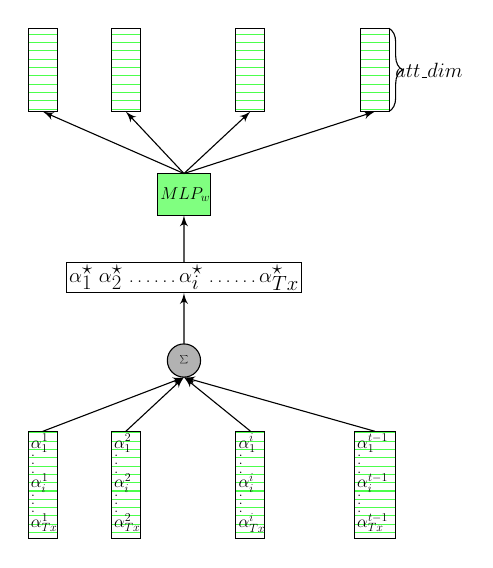
\begin{tikzpicture}[scale=0.3, every node/.style={transform shape, font=\fontsize{40}{40}\selectfont}]
	\node [atts, minimum height = 12em] (alpha1) {$\alpha_{1}^{1}$ \newline . \newline . \newline . \newline $\alpha_{i}^{1}$ \newline . \newline . \newline . \newline $\alpha_{Tx}^{1}$ \newline};
	\node [atts, right of=alpha1, minimum height = 12em] (alpha2) {$\alpha_{1}^{2}$ \newline . \newline . \newline . \newline $\alpha_{i}^{2}$ \newline . \newline . \newline . \newline $\alpha_{Tx}^{2}$ \newline};
	\node [atts, right of=alpha2, node distance = 15em, minimum height = 12em] (alphai) {$\alpha_{1}^{i}$ \newline . \newline . \newline . \newline $\alpha_{i}^{i}$ \newline . \newline . \newline . \newline $\alpha_{Tx}^{i}$ \newline};
	\node [atts, right of=alphai, node distance = 15em, minimum height = 12em, text width = 1.5cm] (alphaTx) {$\alpha_{1}^{t-1}$ \newline . \newline . \newline . \newline $\alpha_{i}^{t-1}$ \newline . \newline . \newline . \newline $\alpha_{Tx}^{t-1}$ \newline};
	\node [round, above of = alphai, xshift = -8em, node distance = 15em] (sum) {$\sum$};
	\path [line] (alpha1.north) to (sum.south);
	\path [line] (alpha2.north) to (sum.south);
	\path [line] (alphai.north) to (sum.south);
	\path [line] (alphaTx.north) to (sum.south);
	\node [draw, above of = sum, node distance = 10em] (alphastar) {$\alpha_{1}^{\star}$ $\alpha_{2}^{\star}$ \dots \dots $\alpha_{i}^{\star}$ \dots \dots $\alpha_{Tx}^{\star}$};
	\node [mlp_att, above of = alphastar, node distance = 10em] (mlp_w) {$MLP_{w}$};
	
	\node [atts, above of = alpha1, node distance = 50em] (alpha1) {};
	\node [atts, right of=alpha1] (alpha2) {};
	\node [atts, right of=alpha2, node distance = 15em] (alphai) {};
	\node [atts, right of=alphai, node distance = 15em] (alphaTx) {};
	
	
	\draw [decorate,decoration={brace,amplitude=5pt, raise=0.5em}] (alphaTx.90) -- (alphaTx.-90) node [black,midway, xshift=6.5em] {\fontsize{25}{10}\selectfont $att\_dim$};
	
	\path [line] (sum.north) to (alphastar.south);
	\path [line] (alphastar.north) to (mlp_w.south);
	\path [line] (mlp_w.north) to (alpha1.south);
	\path [line] (mlp_w.north) to (alpha2.south);
	\path [line] (mlp_w.north) to (alphai.south);
	\path [line] (mlp_w.north) to (alphaTx.south);
	
	
	\end{tikzpicture}
\end{center}
\end{frame}

\begin{frame}[fragile]{Coverage mechanism Attention}
\begin{center}
	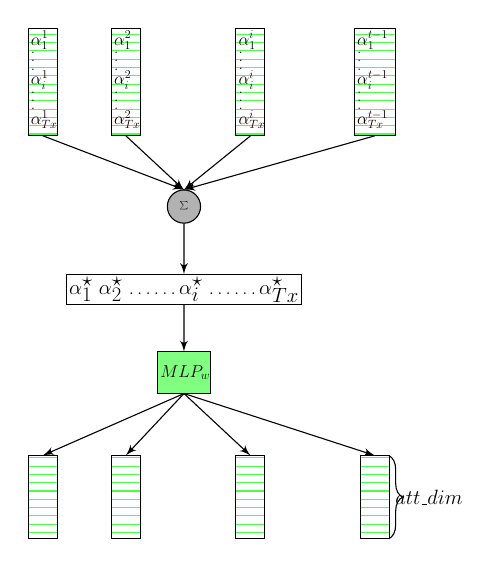
\begin{tikzpicture}[scale=0.3, every node/.style={transform shape, font=\fontsize{40}{40}\selectfont}]
	\node [atts, minimum height = 12em] (alpha1) {$\alpha_{1}^{1}$ \newline . \newline . \newline . \newline $\alpha_{i}^{1}$ \newline . \newline . \newline . \newline $\alpha_{Tx}^{1}$ \newline};
	
	\node [atts, right of=alpha1, minimum height = 12em] (alpha2) {$\alpha_{1}^{2}$ \newline . \newline . \newline . \newline $\alpha_{i}^{2}$ \newline . \newline . \newline . \newline $\alpha_{Tx}^{2}$ \newline};
	
	\node [atts, right of=alpha2, node distance = 15em, minimum height = 12em] (alphai) {$\alpha_{1}^{i}$ \newline . \newline . \newline . \newline $\alpha_{i}^{i}$ \newline . \newline . \newline . \newline $\alpha_{Tx}^{i}$ \newline};
	
	\node [atts, right of=alphai, node distance = 15em, minimum height = 12em, text width = 1.5cm] (alphaTx) {$\alpha_{1}^{t-1}$ \newline . \newline . \newline . \newline $\alpha_{i}^{t-1}$ \newline . \newline . \newline . \newline $\alpha_{Tx}^{t-1}$ \newline};
	
	\node [round, below of = alphai, xshift = -8em, node distance = 15em] (sum) {$\sum$};
	\path [line] (alpha1.south) to (sum.north);
	\path [line] (alpha2.south) to (sum.north);
	\path [line] (alphai.south) to (sum.north);
	\path [line] (alphaTx.south) to (sum.north);
	
	\node [draw, below of = sum, node distance = 10em] (alphastar) {$\alpha_{1}^{\star}$ $\alpha_{2}^{\star}$ \dots \dots $\alpha_{i}^{\star}$ \dots \dots $\alpha_{Tx}^{\star}$};
	\node [mlp_att, below of = alphastar, node distance = 10em] (mlp_w) {$MLP_{w}$};
	
	\node [atts, below of = alpha1, node distance = 50em] (alpha1) {};
	\node [atts, right of=alpha1] (alpha2) {};
	\node [atts, right of=alpha2, node distance = 15em] (alphai) {};
	\node [atts, right of=alphai, node distance = 15em] (alphaTx) {};
	
	
	\draw [decorate,decoration={brace,amplitude=5pt, raise=0.5em}] (alphaTx.90) -- (alphaTx.-90) node [black,midway, xshift=6.5em] {\fontsize{25}{10}\selectfont $att\_dim$};
	
	\path [line] (sum.south) to (alphastar.north);
	\path [line] (alphastar.south) to (mlp_w.north);
	\path [line] (mlp_w.south) to (alpha1.north);
	\path [line] (mlp_w.south) to (alpha2.north);
	\path [line] (mlp_w.south) to (alphai.north);
	\path [line] (mlp_w.south) to (alphaTx.north);
	\end{tikzpicture}
\end{center}
\end{frame}	


\begin{frame}[fragile]{Coverage mechanism Attention}
\begin{center}
	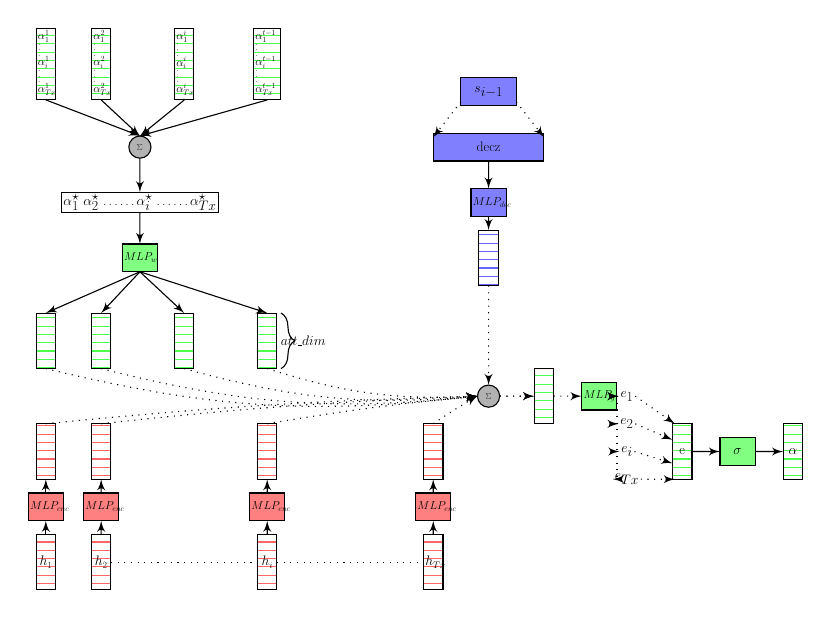
\begin{tikzpicture}[scale=0.2, every node/.style={transform shape, font=\fontsize{40}{40}\selectfont}]
	
	\node [enc_h] (h1) {$h_{1}$};
	\node [enc_h,right of = h1] (h2) {$h_{2}$};
	\node [enc_h,right of = h2, node distance = 30em] (hi) {$h_{i}$};
	\node [enc_h,right of = hi, node distance = 30em] (hTx) {$h_{Tx}$};
	\draw [dotted] (h2.east) to (hi.west);
	\draw [dotted] (hi.east) to (hTx.west);
	
	
	\node [mlp_enc, above of = h1, node distance = 10em] (mlp1) {$MLP_{enc}$};
	\path [line] (h1.north) to (mlp1.south);
	\node [enc_h, above of = mlp1] (he1) {};
	\path [line] (mlp1.north) to (he1.south);
	
	
	\node [mlp_enc, above of = h2, node distance = 10em] (mlp2) {$MLP_{enc}$};
	\path [line] (h2.north) to (mlp2.south);
	\node [enc_h, above of = mlp2] (he2) {};
	\path [line] (mlp2.north) to (he2.south);
	
	
	\node [mlp_enc, above of = hi, node distance = 10em] (mlpi) {$MLP_{enc}$};
	\path [line] (hi.north) to (mlpi.south);
	\node [enc_h, above of = mlpi] (hei) {};
	\path [line] (mlpi.north) to (hei.south);
	
	
	\node [mlp_enc, above of = hTx, node distance = 10em] (mlpTx) {$MLP_{enc}$};
	\path [line] (hTx.north) to (mlpTx.south);
	\node [enc_h, above of = mlpTx] (heTx) {};
	\path [line] (mlpTx.north) to (heTx.south);
	
	
	\node [atts, minimum height = 12em,  above of=he1, node distance = 70em] (alpha1) {$\alpha_{1}^{1}$ \newline . \newline . \newline . \newline $\alpha_{i}^{1}$ \newline . \newline . \newline . \newline $\alpha_{Tx}^{1}$ \newline};
	
	\node [atts, right of=alpha1, minimum height = 12em] (alpha2) {$\alpha_{1}^{2}$ \newline . \newline . \newline . \newline $\alpha_{i}^{2}$ \newline . \newline . \newline . \newline $\alpha_{Tx}^{2}$ \newline};
	
	\node [atts, right of=alpha2, node distance = 15em, minimum height = 12em] (alphai) {$\alpha_{1}^{i}$ \newline . \newline . \newline . \newline $\alpha_{i}^{i}$ \newline . \newline . \newline . \newline $\alpha_{Tx}^{i}$ \newline};
	
	\node [atts, right of=alphai, node distance = 15em, minimum height = 12em, text width = 1.5cm] (alphaTx) {$\alpha_{1}^{t-1}$ \newline . \newline . \newline . \newline $\alpha_{i}^{t-1}$ \newline . \newline . \newline . \newline $\alpha_{Tx}^{t-1}$ \newline};
	
	\node [round, below of = alphai, xshift = -8em, node distance = 15em] (sum) {$\sum$};
	\path [line] (alpha1.south) to (sum.north);
	\path [line] (alpha2.south) to (sum.north);
	\path [line] (alphai.south) to (sum.north);
	\path [line] (alphaTx.south) to (sum.north);
	
	\node [draw, below of = sum, node distance = 10em] (alphastar) {$\alpha_{1}^{\star}$ $\alpha_{2}^{\star}$ \dots \dots $\alpha_{i}^{\star}$ \dots \dots $\alpha_{Tx}^{\star}$};
	\node [mlp_att, below of = alphastar, node distance = 10em] (mlp_w) {$MLP_{w}$};
	
	\node [atts, below of = alpha1, node distance = 50em] (alpha1) {};
	\node [atts, right of=alpha1] (alpha2) {};
	\node [atts, right of=alpha2, node distance = 15em] (alphai) {};
	\node [atts, right of=alphai, node distance = 15em] (alphaTx) {};
	
	
	\draw [decorate,decoration={brace,amplitude=5pt, raise=0.5em}] (alphaTx.90) -- (alphaTx.-90) node [black,midway, xshift=6.5em] {\fontsize{25}{10}\selectfont $att\_dim$};
	
	\path [line] (sum.south) to (alphastar.north);
	\path [line] (alphastar.south) to (mlp_w.north);
	\path [line] (mlp_w.south) to (alpha1.north);
	\path [line] (mlp_w.south) to (alpha2.north);
	\path [line] (mlp_w.south) to (alphai.north);
	\path [line] (mlp_w.south) to (alphaTx.north);
	
	\node [round, above of=heTx, node distance=10em, xshift=10em] (sum1) {$\sum$};
	
	\path [line, dotted] (he1.north) to [bend left=2] (sum1.west);
	\path [line, dotted] (he2.north) to [bend left=2] (sum1.west);
	\path [line, dotted] (hei.north) to [bend left=2] (sum1.west);
	\path [line, dotted] (heTx.north) to [bend left=2] (sum1.west);
	
	
	\node [mlp_dec, right of = mlp_w, node distance = 63em, minimum width = 10em, yshift=30em, font=\fontsize{40}{10}\selectfont] (sim1) {$s_{i-1}$};
	\node [mlp_dec, below of=sim1, minimum width = 20em, font=\fontsize{40}{10}\selectfont] (dec_z) {decz};
	\path [line, dotted] (sim1.200) to (dec_z.170);
	\path [line, dotted] (sim1.-20) to (dec_z.10);
	\node [mlp_dec, below of=dec_z, node distance = 10em] (mlp_dec) {$MLP_{dec}$};
	\path [line] (dec_z) to (mlp_dec);
	\node [dec_z, below of = mlp_dec] (decz_enc) {};
	\path [line] (mlp_dec) to (decz_enc);
	
	\path [line, dotted] (decz_enc.south) to (sum1.north);
	
	%		\path [line, dotted] (ht.east) to [bend left=10] (sum1.110);
	\node [atts, right of=sum1, node distance = 10em] (asdf) {};
	\node [mlp_att, right of=asdf] (mlpg) {$MLP_{g}$};
	\node [right of=mlpg, node distance=5em, font=\fontsize{40}{10}\selectfont] (e1) {$e_1$};
	
	\node [below of=e1, node distance=5em, font=\fontsize{40}{10}\selectfont] (e2) {$e_2$};
	
	\node [below of=e2, node distance=5em, font=\fontsize{40}{10}\selectfont] (ei) {$e_i$};
	
	\node [below of=ei, node distance=5em, font=\fontsize{40}{10}\selectfont] (eTx) {$e_{Tx}$};
	
	\node [atts, right of=ei, font=\fontsize{40}{10}\selectfont] (e) {e};
	
	\path [line, dotted] (e1.east) to (e.105);
	\path [line, dotted] (e2.east) to (e.130);
	\path [line, dotted] (ei.east) to (e.-130);
	\path [line, dotted] (eTx.east) to (e.-105);
	
	\node [mlp_att, right of=e, font=\fontsize{40}{10}\selectfont] (sm) {$\sigma$};
	\path [line] (e.east) to (sm.west);
	
	
	\node [atts, right of=sm, font=\fontsize{40}{10}\selectfont] (alphas) {$\alpha$};
	\path [line] (sm.east) to (alphas.west);
	
	\path [line, dotted] (sum1.east) to (asdf.west);
	\path [line, dotted] (sum1.east) to (asdf.west);
	\path [line, dotted] (asdf.east) to (mlpg.west);
	\path [line, dotted] (mlpg.east) to (e1.west);
	\path [line, dotted] (mlpg.east) to (e1.west);
	\path [line, dotted] (mlpg.east) |- (e2.west);
	\path [line, dotted] (mlpg.east) |- (ei.west);
	\path [line, dotted] (mlpg.east) |- (eTx.west);
	
	\path [line, dotted] (alpha1.south) to [bend right=10] (sum1.west);
	\path [line, dotted] (alpha2.south) to [bend right=10] (sum1.west);
	\path [line, dotted] (alphai.south) to [bend right=10] (sum1.west);
	\path [line, dotted] (alphaTx.south) to [bend right=10] (sum1.west);
	\end{tikzpicture}
\end{center}
\end{frame}


\begin{frame}[fragile]{Coverage mechanism Attention}
\begin{center}
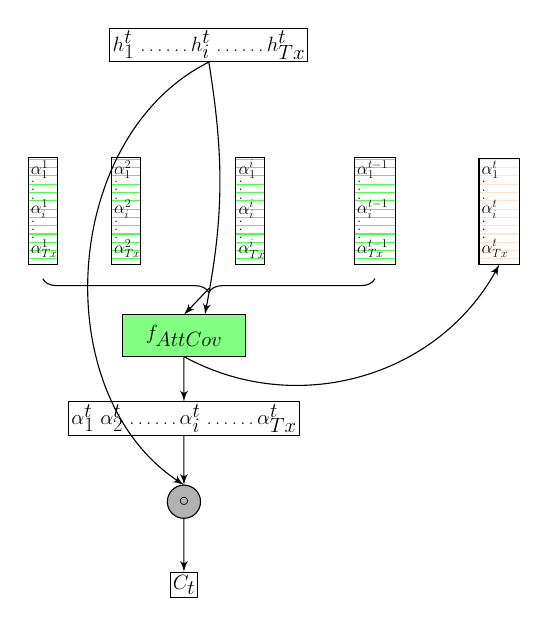
\begin{tikzpicture}[scale=0.3, every node/.style={transform shape, font=\fontsize{40}{40}\selectfont}]
\node [draw] (ht) {$h_{1}^{t}$ \dots \dots $h_{i}^{t}$ \dots \dots $h_{Tx}^{t}$};

\node [atts, below of = ht, xshift=-20em, node distance = 20em] (alpha1) {$\alpha_{1}^{1}$ \newline . \newline . \newline . \newline $\alpha_{i}^{1}$ \newline . \newline . \newline . \newline $\alpha_{Tx}^{1}$ \newline};
\node [atts, right of=alpha1, minimum height = 12em] (alpha2) {$\alpha_{1}^{2}$ \newline . \newline . \newline . \newline $\alpha_{i}^{2}$ \newline . \newline . \newline . \newline $\alpha_{Tx}^{2}$ \newline};
\node [atts, right of=alpha2, node distance = 15em, minimum height = 12em] (alphai) {$\alpha_{1}^{i}$ \newline . \newline . \newline . \newline $\alpha_{i}^{i}$ \newline . \newline . \newline . \newline $\alpha_{Tx}^{i}$ \newline};
\node [atts, right of=alphai, node distance = 15em, minimum height = 12em, text width = 1.5cm] (alphaTx) {$\alpha_{1}^{t-1}$ \newline . \newline . \newline . \newline $\alpha_{i}^{t-1}$ \newline . \newline . \newline . \newline $\alpha_{Tx}^{t-1}$ \newline};

\node [mlp_att, below of= alphai, xshift=-8em, font=\fontsize{60}{60}\selectfont, text width = 5cm, node distance = 15em] (attcov) {$f_{AttCov}$};

\node [draw, below of = attcov, node distance = 10em] (alphastar) {$\alpha_{1}^{t}$ $\alpha_{2}^{t}$ \dots \dots $\alpha_{i}^{t}$ \dots \dots $\alpha_{Tx}^{t}$};

\draw [decorate,decoration={brace,amplitude=5pt, raise=0.5em, mirror}] (alpha1.south) -- (alphaTx.south) node [black,midway, yshift = -2.5em] (t) {};

\path [line] (t.south) to (attcov.north);

\path [line] (ht.south) to [bend left=10] (attcov.45);
\path [line] (attcov.south) to (alphastar);

\node [atts, right of=alphaTx,pattern color= orange!20, node distance = 15em, minimum height = 12em, text width = 1.5cm] (alphat) {$\alpha_{1}^{t}$ \newline . \newline . \newline . \newline $\alpha_{i}^{t}$ \newline . \newline . \newline . \newline $\alpha_{Tx}^{t}$ \newline};

\path [line] (attcov.south) to [bend right=45](alphat.south);
\node [round, below of=alphastar, node distance = 10em] (dot) {$\circ$};
\path [line] (ht.south) to [bend right=60](dot.north);
\path [line] (alphastar.south) to (dot.north);

\node [draw, below of = dot, node distance = 10em] (ct) {$C_{t}$};

\path [line] (dot.south) to (ct.north);

\end{tikzpicture}
\end{center}
\end{frame}







\section{Coverage mechanism location aware Attention}


\begin{frame}[fragile]{Coverage mechanism location aware Attention}
\begin{center}
	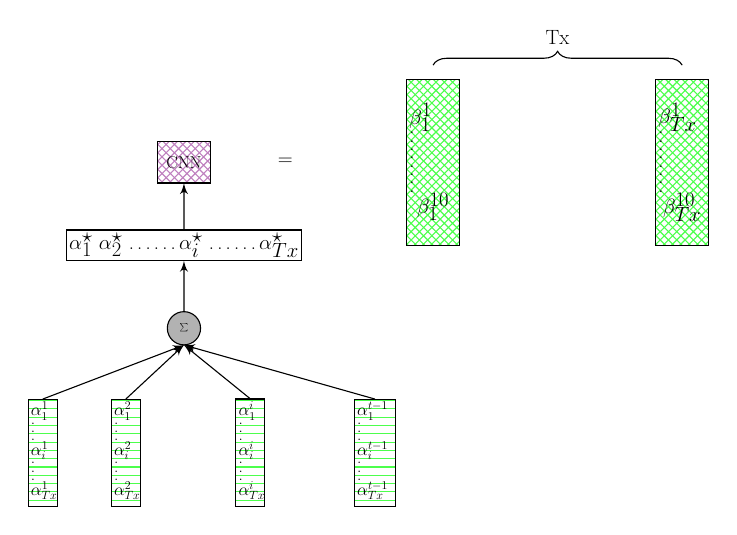
\begin{tikzpicture}[scale=0.3, every node/.style={transform shape, font=\fontsize{40}{40}\selectfont}]
	\node [atts, minimum height = 12em] (alpha1) {$\alpha_{1}^{1}$ \newline . \newline . \newline . \newline $\alpha_{i}^{1}$ \newline . \newline . \newline . \newline $\alpha_{Tx}^{1}$ \newline};
	\node [atts, right of=alpha1, minimum height = 12em] (alpha2) {$\alpha_{1}^{2}$ \newline . \newline . \newline . \newline $\alpha_{i}^{2}$ \newline . \newline . \newline . \newline $\alpha_{Tx}^{2}$ \newline};
	\node [atts, right of=alpha2, node distance = 15em, minimum height = 12em] (alphai) {$\alpha_{1}^{i}$ \newline . \newline . \newline . \newline $\alpha_{i}^{i}$ \newline . \newline . \newline . \newline $\alpha_{Tx}^{i}$ \newline};
	\node [atts, right of=alphai, node distance = 15em, minimum height = 12em, text width = 1.5cm] (alphaTx) {$\alpha_{1}^{t-1}$ \newline . \newline . \newline . \newline $\alpha_{i}^{t-1}$ \newline . \newline . \newline . \newline $\alpha_{Tx}^{t-1}$ \newline};
	\node [round, above of = alphai, xshift = -8em, node distance = 15em] (sum) {$\sum$};
	\path [line] (alpha1.north) to (sum.south);
	\path [line] (alpha2.north) to (sum.south);
	\path [line] (alphai.north) to (sum.south);
	\path [line] (alphaTx.north) to (sum.south);
	\node [draw, above of = sum, node distance = 10em] (alphastar) {$\alpha_{1}^{\star}$ $\alpha_{2}^{\star}$ \dots \dots $\alpha_{i}^{\star}$ \dots \dots $\alpha_{Tx}^{\star}$};
	
	\path [line] (sum.north) to (alphastar.south);
	
	\node [cnn, above of =alphastar] (cnn1) {CNN};
	
	\node [atts, right of = cnn1, pattern=crosshatch, node distance = 50em, minimum height = 20em, text width=2cm,font=\fontsize{40}{10}\selectfont, xshift=-20em] (b1) {$\beta_{1}^{1}$ \newline . \newline . \newline . \newline . \newline . \newline . \newline . \newline . \newline $\beta_{1}^{10}$} ;
	
	\node [atts, right of = b1, pattern=crosshatch, node distance = 30em, minimum height = 20em, text width=2cm,font=\fontsize{40}{10}\selectfont] (b2) {$\beta_{Tx}^{1}$ \newline . \newline . \newline . \newline . \newline . \newline . \newline . \newline . \newline $\beta_{Tx}^{10}$} ;
	
	\draw [decorate,decoration={brace,amplitude=5pt, raise=0.5em}] (b1.north) -- (b2.north) node [black,midway, yshift=5em] {\fontsize{40}{10}\selectfont Tx};
	
	
	\node [right of = cnn1, node distance = 12em, font=\fontsize{40}{10}\selectfont] (eq) {$\,=$};
	\path [line] (alphastar.north) to (cnn1.south);
	\end{tikzpicture}
\end{center}
\end{frame}



\begin{frame}[fragile]{Coverage mechanism location aware Attention}
\begin{center}
	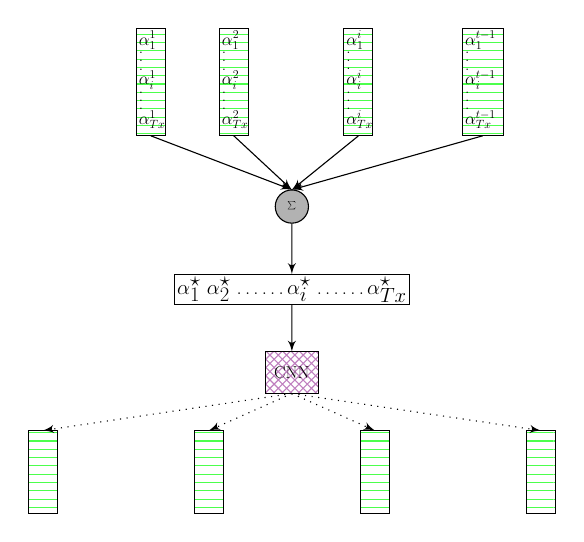
\begin{tikzpicture}[scale=0.3, every node/.style={transform shape, font=\fontsize{40}{40}\selectfont}]
	
	\node [atts, minimum height = 12em] (alpha1) {$\alpha_{1}^{1}$ \newline . \newline . \newline . \newline $\alpha_{i}^{1}$ \newline . \newline . \newline . \newline $\alpha_{Tx}^{1}$ \newline};
	
	\node [atts, right of=alpha1, minimum height = 12em] (alpha2) {$\alpha_{1}^{2}$ \newline . \newline . \newline . \newline $\alpha_{i}^{2}$ \newline . \newline . \newline . \newline $\alpha_{Tx}^{2}$ \newline};
	
	\node [atts, right of=alpha2, node distance = 15em, minimum height = 12em] (alphai) {$\alpha_{1}^{i}$ \newline . \newline . \newline . \newline $\alpha_{i}^{i}$ \newline . \newline . \newline . \newline $\alpha_{Tx}^{i}$ \newline};
	
	\node [atts, right of=alphai, node distance = 15em, minimum height = 12em, text width = 1.5cm] (alphaTx) {$\alpha_{1}^{t-1}$ \newline . \newline . \newline . \newline $\alpha_{i}^{t-1}$ \newline . \newline . \newline . \newline $\alpha_{Tx}^{t-1}$ \newline};
	
	\node [round, below of = alphai, xshift = -8em, node distance = 15em] (sum) {$\sum$};
	
	\path [line] (alpha1.south) to (sum.north);
	\path [line] (alpha2.south) to (sum.north);
	\path [line] (alphai.south) to (sum.north);
	\path [line] (alphaTx.south) to (sum.north);
	
	\node [draw, below of = sum, node distance = 10em] (alphastar) {$\alpha_{1}^{\star}$ $\alpha_{2}^{\star}$ \dots \dots $\alpha_{i}^{\star}$ \dots \dots $\alpha_{Tx}^{\star}$};
	
	\path [line] (sum.south) to (alphastar.north);
	
	\node [cnn, below of =alphastar] (cnn1) {CNN};
	
	\node [atts, below of = cnn1, node distance = 12em, xshift=-30em] (alpha1) {};
	\node [atts, right of = alpha1, node distance = 20em] (alpha2) {};
	\node [atts, right of = alpha2, node distance = 20em] (alphai) {};
	\node [atts, right of = alphai, node distance = 20em] (alphaTx) {};
	\path [line, dotted] (cnn1.south) to (alpha1.north);
	\path [line, dotted] (cnn1.south) to (alpha2.north);
	\path [line, dotted] (cnn1.south) to (alphai.north);
	\path [line, dotted] (cnn1.south) to (alphaTx.north);
	
	
	\path [line] (alphastar.south) to (cnn1.north);
	\end{tikzpicture}
\end{center}
\end{frame}



\begin{frame}[fragile]{Coverage mechanism location aware Attention}
\begin{center}
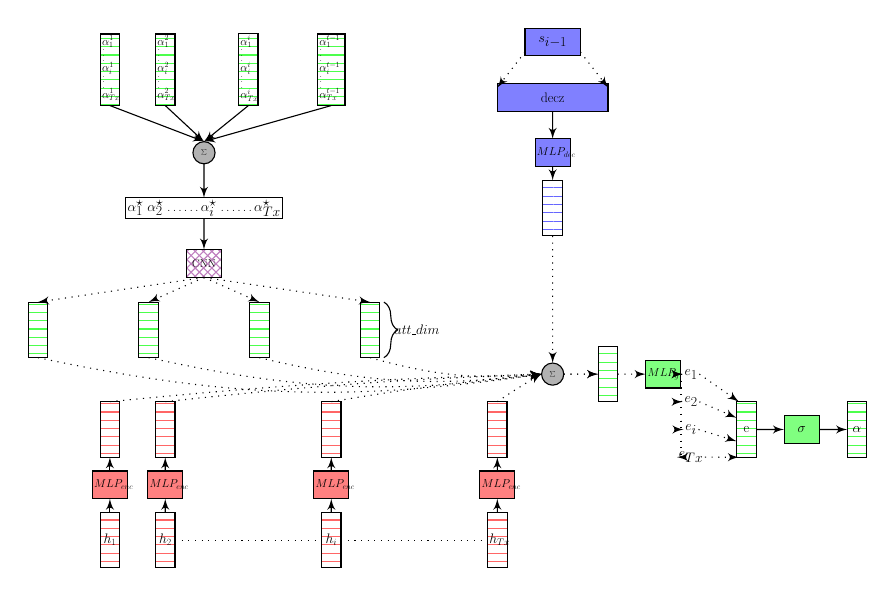
\begin{tikzpicture}[scale=0.2, every node/.style={transform shape, font=\fontsize{40}{40}\selectfont}]

\node [enc_h] (h1) {$h_{1}$};
\node [enc_h,right of = h1] (h2) {$h_{2}$};
\node [enc_h,right of = h2, node distance = 30em] (hi) {$h_{i}$};
\node [enc_h,right of = hi, node distance = 30em] (hTx) {$h_{Tx}$};
\draw [dotted] (h2.east) to (hi.west);
\draw [dotted] (hi.east) to (hTx.west);


\node [mlp_enc, above of = h1, node distance = 10em] (mlp1) {$MLP_{enc}$};
\path [line] (h1.north) to (mlp1.south);
\node [enc_h, above of = mlp1] (he1) {};
\path [line] (mlp1.north) to (he1.south);


\node [mlp_enc, above of = h2, node distance = 10em] (mlp2) {$MLP_{enc}$};
\path [line] (h2.north) to (mlp2.south);
\node [enc_h, above of = mlp2] (he2) {};
\path [line] (mlp2.north) to (he2.south);


\node [mlp_enc, above of = hi, node distance = 10em] (mlpi) {$MLP_{enc}$};
\path [line] (hi.north) to (mlpi.south);
\node [enc_h, above of = mlpi] (hei) {};
\path [line] (mlpi.north) to (hei.south);


\node [mlp_enc, above of = hTx, node distance = 10em] (mlpTx) {$MLP_{enc}$};
\path [line] (hTx.north) to (mlpTx.south);
\node [enc_h, above of = mlpTx] (heTx) {};
\path [line] (mlpTx.north) to (heTx.south);




\node [atts, minimum height = 12em,  above of=he1, node distance = 65em] (alpha1) {$\alpha_{1}^{1}$ \newline . \newline . \newline . \newline $\alpha_{i}^{1}$ \newline . \newline . \newline . \newline $\alpha_{Tx}^{1}$ \newline};

\node [atts, right of=alpha1, minimum height = 12em] (alpha2) {$\alpha_{1}^{2}$ \newline . \newline . \newline . \newline $\alpha_{i}^{2}$ \newline . \newline . \newline . \newline $\alpha_{Tx}^{2}$ \newline};

\node [atts, right of=alpha2, node distance = 15em, minimum height = 12em] (alphai) {$\alpha_{1}^{i}$ \newline . \newline . \newline . \newline $\alpha_{i}^{i}$ \newline . \newline . \newline . \newline $\alpha_{Tx}^{i}$ \newline};

\node [atts, right of=alphai, node distance = 15em, minimum height = 12em, text width = 1.5cm] (alphaTx) {$\alpha_{1}^{t-1}$ \newline . \newline . \newline . \newline $\alpha_{i}^{t-1}$ \newline . \newline . \newline . \newline $\alpha_{Tx}^{t-1}$ \newline};

\node [round, below of = alphai, xshift = -8em, node distance = 15em] (sum) {$\sum$};

\path [line] (alpha1.south) to (sum.north);
\path [line] (alpha2.south) to (sum.north);
\path [line] (alphai.south) to (sum.north);
\path [line] (alphaTx.south) to (sum.north);

\node [draw, below of = sum, node distance = 10em] (alphastar) {$\alpha_{1}^{\star}$ $\alpha_{2}^{\star}$ \dots \dots $\alpha_{i}^{\star}$ \dots \dots $\alpha_{Tx}^{\star}$};

\path [line] (sum.south) to (alphastar.north);

\node [cnn, below of =alphastar] (cnn1) {CNN};

\node [atts, below of = cnn1, node distance = 12em, xshift=-30em] (alpha1) {};
\node [atts, right of = alpha1, node distance = 20em] (alpha2) {};
\node [atts, right of = alpha2, node distance = 20em] (alphai) {};
\node [atts, right of = alphai, node distance = 20em] (alphaTx) {};
\path [line, dotted] (cnn1.south) to (alpha1.north);
\path [line, dotted] (cnn1.south) to (alpha2.north);
\path [line, dotted] (cnn1.south) to (alphai.north);
\path [line, dotted] (cnn1.south) to (alphaTx.north);
\path [line] (alphastar.south) to (cnn1.north);

\draw [decorate,decoration={brace,amplitude=5pt, raise=0.5em}] (alphaTx.90) -- (alphaTx.-90) node [black,midway, xshift=8.5em] {\fontsize{25}{10}\selectfont $att\_dim$};


\node [round, above of=heTx, node distance=10em, xshift=10em] (sum1) {$\sum$};

\path [line, dotted] (he1.north) to [bend left=2] (sum1.west);
\path [line, dotted] (he2.north) to [bend left=2] (sum1.west);
\path [line, dotted] (hei.north) to [bend left=2] (sum1.west);
\path [line, dotted] (heTx.north) to [bend left=2] (sum1.west);


\node [mlp_dec, right of = alphastar, node distance = 63em, minimum width = 10em, yshift=30em, font=\fontsize{40}{10}\selectfont] (sim1) {$s_{i-1}$};
\node [mlp_dec, below of=sim1, minimum width = 20em, font=\fontsize{40}{10}\selectfont] (dec_z) {decz};
\path [line, dotted] (sim1.200) to (dec_z.170);
\path [line, dotted] (sim1.-20) to (dec_z.10);
\node [mlp_dec, below of=dec_z, node distance = 10em] (mlp_dec) {$MLP_{dec}$};
\path [line] (dec_z) to (mlp_dec);
\node [dec_z, below of = mlp_dec] (decz_enc) {};
\path [line] (mlp_dec) to (decz_enc);

\path [line, dotted] (decz_enc.south) to (sum1.north);

%		\path [line, dotted] (ht.east) to [bend left=10] (sum1.110);
\node [atts, right of=sum1, node distance = 10em] (asdf) {};
\node [mlp_att, right of=asdf] (mlpg) {$MLP_{g}$};
\node [right of=mlpg, node distance=5em, font=\fontsize{40}{10}\selectfont] (e1) {$e_1$};

\node [below of=e1, node distance=5em, font=\fontsize{40}{10}\selectfont] (e2) {$e_2$};

\node [below of=e2, node distance=5em, font=\fontsize{40}{10}\selectfont] (ei) {$e_i$};

\node [below of=ei, node distance=5em, font=\fontsize{40}{10}\selectfont] (eTx) {$e_{Tx}$};

\node [atts, right of=ei, font=\fontsize{40}{10}\selectfont] (e) {e};

\path [line, dotted] (e1.east) to (e.105);
\path [line, dotted] (e2.east) to (e.130);
\path [line, dotted] (ei.east) to (e.-130);
\path [line, dotted] (eTx.east) to (e.-105);

\node [mlp_att, right of=e, font=\fontsize{40}{10}\selectfont] (sm) {$\sigma$};
\path [line] (e.east) to (sm.west);


\node [atts, right of=sm, font=\fontsize{40}{10}\selectfont] (alphas) {$\alpha$};
\path [line] (sm.east) to (alphas.west);

\path [line, dotted] (sum1.east) to (asdf.west);
\path [line, dotted] (sum1.east) to (asdf.west);
\path [line, dotted] (asdf.east) to (mlpg.west);
\path [line, dotted] (mlpg.east) to (e1.west);
\path [line, dotted] (mlpg.east) to (e1.west);
\path [line, dotted] (mlpg.east) |- (e2.west);
\path [line, dotted] (mlpg.east) |- (ei.west);
\path [line, dotted] (mlpg.east) |- (eTx.west);

\path [line, dotted] (alpha1.south) to [bend right=10] (sum1.west);
\path [line, dotted] (alpha2.south) to [bend right=10] (sum1.west);
\path [line, dotted] (alphai.south) to [bend right=10] (sum1.west);
\path [line, dotted] (alphaTx.south) to [bend right=10] (sum1.west);
\end{tikzpicture}
\end{center}
\end{frame}



\begin{frame}[fragile]{Coverage mechanism location aware Attention}
\begin{center}
	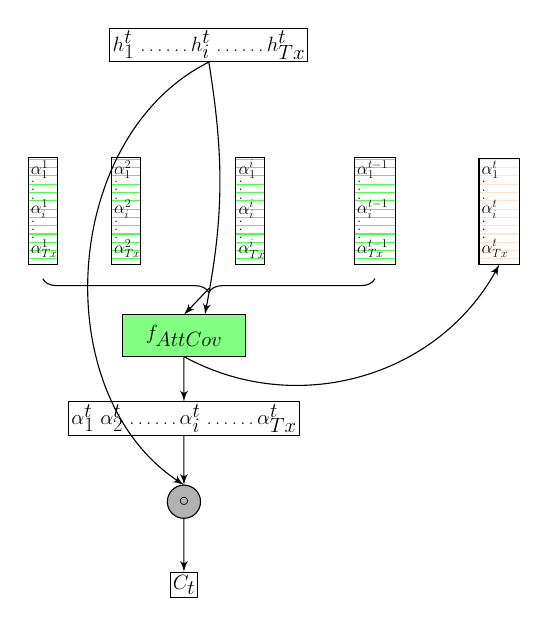
\begin{tikzpicture}[scale=0.3, every node/.style={transform shape, font=\fontsize{40}{40}\selectfont}]
	
	\node [draw] (ht) {$h_{1}^{t}$ \dots \dots $h_{i}^{t}$ \dots \dots $h_{Tx}^{t}$};
	
	\node [atts, below of = ht, xshift=-20em, node distance = 20em] (alpha1) {$\alpha_{1}^{1}$ \newline . \newline . \newline . \newline $\alpha_{i}^{1}$ \newline . \newline . \newline . \newline $\alpha_{Tx}^{1}$ \newline};
	\node [atts, right of=alpha1, minimum height = 12em] (alpha2) {$\alpha_{1}^{2}$ \newline . \newline . \newline . \newline $\alpha_{i}^{2}$ \newline . \newline . \newline . \newline $\alpha_{Tx}^{2}$ \newline};
	\node [atts, right of=alpha2, node distance = 15em, minimum height = 12em] (alphai) {$\alpha_{1}^{i}$ \newline . \newline . \newline . \newline $\alpha_{i}^{i}$ \newline . \newline . \newline . \newline $\alpha_{Tx}^{i}$ \newline};
	\node [atts, right of=alphai, node distance = 15em, minimum height = 12em, text width = 1.5cm] (alphaTx) {$\alpha_{1}^{t-1}$ \newline . \newline . \newline . \newline $\alpha_{i}^{t-1}$ \newline . \newline . \newline . \newline $\alpha_{Tx}^{t-1}$ \newline};
	
	\node [mlp_att, below of= alphai, xshift=-8em, font=\fontsize{60}{60}\selectfont, text width = 5cm, node distance = 15em] (attcov) {$f_{AttCov}$};
	
	\node [draw, below of = attcov, node distance = 10em] (alphastar) {$\alpha_{1}^{t}$ $\alpha_{2}^{t}$ \dots \dots $\alpha_{i}^{t}$ \dots \dots $\alpha_{Tx}^{t}$};
	
	\draw [decorate,decoration={brace,amplitude=5pt, raise=0.5em, mirror}] (alpha1.south) -- (alphaTx.south) node [black,midway, yshift = -2.5em] (t) {};
	
	\path [line] (t.south) to (attcov.north);
	
	\path [line] (ht.south) to [bend left=10] (attcov.45);
	\path [line] (attcov.south) to (alphastar);
	
	\node [atts, right of=alphaTx,pattern color= orange!20, node distance = 15em, minimum height = 12em, text width = 1.5cm] (alphat) {$\alpha_{1}^{t}$ \newline . \newline . \newline . \newline $\alpha_{i}^{t}$ \newline . \newline . \newline . \newline $\alpha_{Tx}^{t}$ \newline};
	
	\path [line] (attcov.south) to [bend right=45](alphat.south);
	\node [round, below of=alphastar, node distance = 10em] (dot) {$\circ$};
	\path [line] (ht.south) to [bend right=60](dot.north);
	\path [line] (alphastar.south) to (dot.north);
	
	\node [draw, below of = dot, node distance = 10em] (ct) {$C_{t}$};
	
	\path [line] (dot.south) to (ct.north);
	
	\end{tikzpicture}
\end{center}
\end{frame}

\end{document}